\documentclass[]{book}
\usepackage{lmodern}
\usepackage{amssymb,amsmath}
\usepackage{ifxetex,ifluatex}
\usepackage{fixltx2e} % provides \textsubscript
\ifnum 0\ifxetex 1\fi\ifluatex 1\fi=0 % if pdftex
  \usepackage[T1]{fontenc}
  \usepackage[utf8]{inputenc}
\else % if luatex or xelatex
  \ifxetex
    \usepackage{mathspec}
  \else
    \usepackage{fontspec}
  \fi
  \defaultfontfeatures{Ligatures=TeX,Scale=MatchLowercase}
\fi
% use upquote if available, for straight quotes in verbatim environments
\IfFileExists{upquote.sty}{\usepackage{upquote}}{}
% use microtype if available
\IfFileExists{microtype.sty}{%
\usepackage{microtype}
\UseMicrotypeSet[protrusion]{basicmath} % disable protrusion for tt fonts
}{}
\usepackage[margin=1in]{geometry}
\usepackage{hyperref}
\hypersetup{unicode=true,
            pdftitle={Inapplicable data},
            pdfauthor={Martin Brazeau (m.brazeau@imperial.ac.uk), Thomas Guillerme (guillert@tcd.ie) and Martin Smith (martin.smith@durham.ac.uk)},
            pdfborder={0 0 0},
            breaklinks=true}
\urlstyle{same}  % don't use monospace font for urls
\usepackage{natbib}
\bibliographystyle{plainnat}
\usepackage{color}
\usepackage{fancyvrb}
\newcommand{\VerbBar}{|}
\newcommand{\VERB}{\Verb[commandchars=\\\{\}]}
\DefineVerbatimEnvironment{Highlighting}{Verbatim}{commandchars=\\\{\}}
% Add ',fontsize=\small' for more characters per line
\usepackage{framed}
\definecolor{shadecolor}{RGB}{248,248,248}
\newenvironment{Shaded}{\begin{snugshade}}{\end{snugshade}}
\newcommand{\KeywordTok}[1]{\textcolor[rgb]{0.13,0.29,0.53}{\textbf{#1}}}
\newcommand{\DataTypeTok}[1]{\textcolor[rgb]{0.13,0.29,0.53}{#1}}
\newcommand{\DecValTok}[1]{\textcolor[rgb]{0.00,0.00,0.81}{#1}}
\newcommand{\BaseNTok}[1]{\textcolor[rgb]{0.00,0.00,0.81}{#1}}
\newcommand{\FloatTok}[1]{\textcolor[rgb]{0.00,0.00,0.81}{#1}}
\newcommand{\ConstantTok}[1]{\textcolor[rgb]{0.00,0.00,0.00}{#1}}
\newcommand{\CharTok}[1]{\textcolor[rgb]{0.31,0.60,0.02}{#1}}
\newcommand{\SpecialCharTok}[1]{\textcolor[rgb]{0.00,0.00,0.00}{#1}}
\newcommand{\StringTok}[1]{\textcolor[rgb]{0.31,0.60,0.02}{#1}}
\newcommand{\VerbatimStringTok}[1]{\textcolor[rgb]{0.31,0.60,0.02}{#1}}
\newcommand{\SpecialStringTok}[1]{\textcolor[rgb]{0.31,0.60,0.02}{#1}}
\newcommand{\ImportTok}[1]{#1}
\newcommand{\CommentTok}[1]{\textcolor[rgb]{0.56,0.35,0.01}{\textit{#1}}}
\newcommand{\DocumentationTok}[1]{\textcolor[rgb]{0.56,0.35,0.01}{\textbf{\textit{#1}}}}
\newcommand{\AnnotationTok}[1]{\textcolor[rgb]{0.56,0.35,0.01}{\textbf{\textit{#1}}}}
\newcommand{\CommentVarTok}[1]{\textcolor[rgb]{0.56,0.35,0.01}{\textbf{\textit{#1}}}}
\newcommand{\OtherTok}[1]{\textcolor[rgb]{0.56,0.35,0.01}{#1}}
\newcommand{\FunctionTok}[1]{\textcolor[rgb]{0.00,0.00,0.00}{#1}}
\newcommand{\VariableTok}[1]{\textcolor[rgb]{0.00,0.00,0.00}{#1}}
\newcommand{\ControlFlowTok}[1]{\textcolor[rgb]{0.13,0.29,0.53}{\textbf{#1}}}
\newcommand{\OperatorTok}[1]{\textcolor[rgb]{0.81,0.36,0.00}{\textbf{#1}}}
\newcommand{\BuiltInTok}[1]{#1}
\newcommand{\ExtensionTok}[1]{#1}
\newcommand{\PreprocessorTok}[1]{\textcolor[rgb]{0.56,0.35,0.01}{\textit{#1}}}
\newcommand{\AttributeTok}[1]{\textcolor[rgb]{0.77,0.63,0.00}{#1}}
\newcommand{\RegionMarkerTok}[1]{#1}
\newcommand{\InformationTok}[1]{\textcolor[rgb]{0.56,0.35,0.01}{\textbf{\textit{#1}}}}
\newcommand{\WarningTok}[1]{\textcolor[rgb]{0.56,0.35,0.01}{\textbf{\textit{#1}}}}
\newcommand{\AlertTok}[1]{\textcolor[rgb]{0.94,0.16,0.16}{#1}}
\newcommand{\ErrorTok}[1]{\textcolor[rgb]{0.64,0.00,0.00}{\textbf{#1}}}
\newcommand{\NormalTok}[1]{#1}
\usepackage{longtable,booktabs}
\usepackage{graphicx,grffile}
\makeatletter
\def\maxwidth{\ifdim\Gin@nat@width>\linewidth\linewidth\else\Gin@nat@width\fi}
\def\maxheight{\ifdim\Gin@nat@height>\textheight\textheight\else\Gin@nat@height\fi}
\makeatother
% Scale images if necessary, so that they will not overflow the page
% margins by default, and it is still possible to overwrite the defaults
% using explicit options in \includegraphics[width, height, ...]{}
\setkeys{Gin}{width=\maxwidth,height=\maxheight,keepaspectratio}
\IfFileExists{parskip.sty}{%
\usepackage{parskip}
}{% else
\setlength{\parindent}{0pt}
\setlength{\parskip}{6pt plus 2pt minus 1pt}
}
\setlength{\emergencystretch}{3em}  % prevent overfull lines
\providecommand{\tightlist}{%
  \setlength{\itemsep}{0pt}\setlength{\parskip}{0pt}}
\setcounter{secnumdepth}{5}
% Redefines (sub)paragraphs to behave more like sections
\ifx\paragraph\undefined\else
\let\oldparagraph\paragraph
\renewcommand{\paragraph}[1]{\oldparagraph{#1}\mbox{}}
\fi
\ifx\subparagraph\undefined\else
\let\oldsubparagraph\subparagraph
\renewcommand{\subparagraph}[1]{\oldsubparagraph{#1}\mbox{}}
\fi

%%% Use protect on footnotes to avoid problems with footnotes in titles
\let\rmarkdownfootnote\footnote%
\def\footnote{\protect\rmarkdownfootnote}

%%% Change title format to be more compact
\usepackage{titling}

% Create subtitle command for use in maketitle
\newcommand{\subtitle}[1]{
  \posttitle{
    \begin{center}\large#1\end{center}
    }
}

\setlength{\droptitle}{-2em}
  \title{Inapplicable data}
  \pretitle{\vspace{\droptitle}\centering\huge}
  \posttitle{\par}
  \author{Martin Brazeau
(\href{mailto:m.brazeau@imperial.ac.uk}{\nolinkurl{m.brazeau@imperial.ac.uk}}),
Thomas Guillerme
(\href{mailto:guillert@tcd.ie}{\nolinkurl{guillert@tcd.ie}}) and Martin
Smith
(\href{mailto:martin.smith@durham.ac.uk}{\nolinkurl{martin.smith@durham.ac.uk}})}
  \preauthor{\centering\large\emph}
  \postauthor{\par}
  \predate{\centering\large\emph}
  \postdate{\par}
  \date{2018-04-17}

\usepackage{booktabs}

\usepackage{amsthm}
\newtheorem{theorem}{Theorem}[chapter]
\newtheorem{lemma}{Lemma}[chapter]
\theoremstyle{definition}
\newtheorem{definition}{Definition}[chapter]
\newtheorem{corollary}{Corollary}[chapter]
\newtheorem{proposition}{Proposition}[chapter]
\theoremstyle{definition}
\newtheorem{example}{Example}[chapter]
\theoremstyle{definition}
\newtheorem{exercise}{Exercise}[chapter]
\theoremstyle{remark}
\newtheorem*{remark}{Remark}
\newtheorem*{solution}{Solution}
\begin{document}
\maketitle

{
\setcounter{tocdepth}{1}
\tableofcontents
}
\hypertarget{inapplicable-data-in-a-parsimony-setting}{%
\chapter*{Inapplicable data in a parsimony
setting}\label{inapplicable-data-in-a-parsimony-setting}}
\addcontentsline{toc}{chapter}{Inapplicable data in a parsimony setting}

This document provides a detailed explanation of the algorithm for
handling inapplicable data proposed by \citet{Brazeau2018}.

We first discuss how the \protect\hyperlink{fitch}{Fitch algorithm}
works and introduce the \protect\hyperlink{problems}{problems} that it
encounters in the face of inapplicable character states.

We then introduce our \protect\hyperlink{solution}{solution}, a new
\protect\hyperlink{algorithm}{algorithm}, implemented in various
\protect\hyperlink{software}{software packages}, and discuss its
implications for the coding of \protect\hyperlink{coding}{characters}
and \protect\hyperlink{ambiguity}{ambiguity}.

We close with some \protect\hyperlink{examples}{example} trees that
demonstrate how our algorithm behaves in more complicated cases.

\hypertarget{fitch}{%
\chapter{The Fitch algorithm}\label{fitch}}

This algorithm was proposed by Fitch \citeyearpar{Fitch1971} and is
implemented in many phylogenetic softwares based on maximum parsimony
\citep{swofford2001paup, Goloboff2016} or probabilistic methods
\citep{Ronquist2012mrbayes, Stamatakis2014}. The procedure is simple and
elegant and entails going down the tree to count the number of
transformations, and then going back up the tree to finalise the
ancestral state reconstructions.

The way the algorithm goes up and down depends on the software, but
often employs a \emph{traversal}: a recursive function that can visit
all tips and nodes in a logical fashion. For example, consider the
following tree:

\begin{figure}
\centering
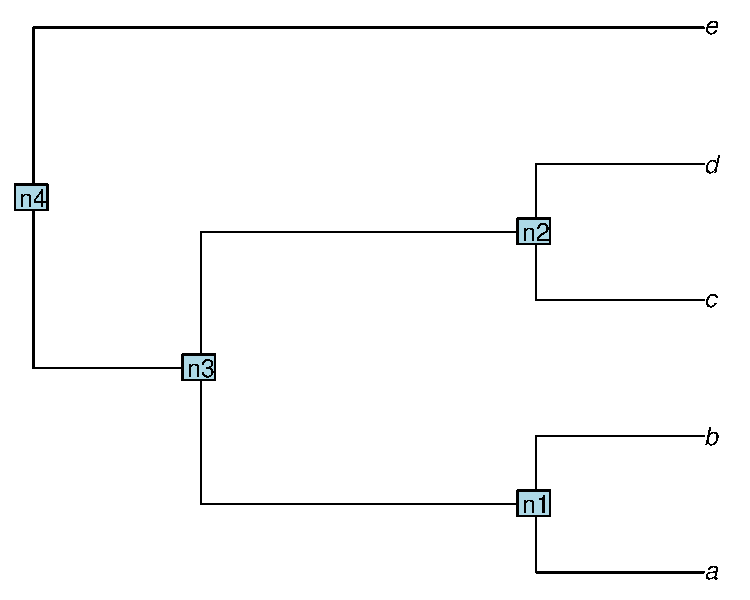
\includegraphics{Inapplicable_data_files/figure-latex/unnamed-chunk-2-1.pdf}
\caption{\label{fig:unnamed-chunk-2}A five-tip tree}
\end{figure}

A downpass traversal will first evaluate the first cherry (or pair of
taxa) (\texttt{A} below), then save the results in \texttt{n1} and
evaluate the second pair of tips/nodes (\texttt{B}), saving the results
in \texttt{n2}, proceeding until all the nodes/tips are visited.

\begin{figure}
\centering
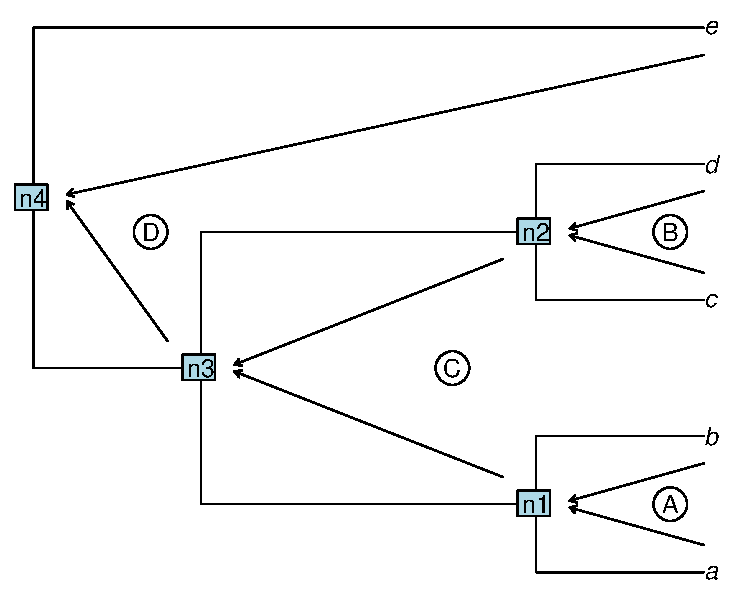
\includegraphics{Inapplicable_data_files/figure-latex/unnamed-chunk-3-1.pdf}
\caption{\label{fig:unnamed-chunk-3}Downpass traversal}
\end{figure}

An uppass traversal works identically but in the other direction, going
from the nodes towards the tips.

\begin{figure}
\centering
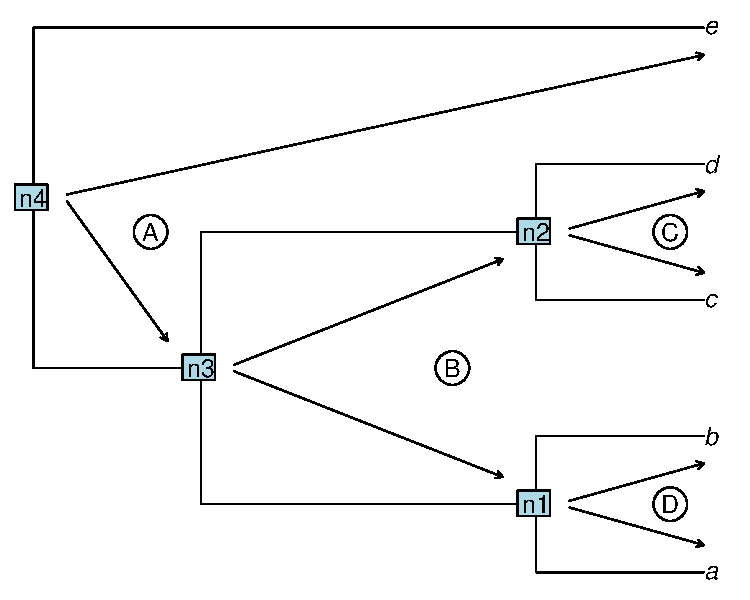
\includegraphics{Inapplicable_data_files/figure-latex/unnamed-chunk-4-1.pdf}
\caption{\label{fig:unnamed-chunk-4}Uppass traversal}
\end{figure}

In both traversals, the sequence in which nodes are visited (i.e.~which
cherry to pick first in a downpass traversal, or whether to continue
left or right in an uppass traversal) is arbitrary, provided that all
tips and nodes are eventually visited.

Now let's consider a more complex tree
\texttt{((((a,\ b),\ c),\ d),\ (e,\ (f,\ (g,\ h))));} with a binary
character distributed ((((1, 0), 0), 1), (1, (0, (0, 1)))):

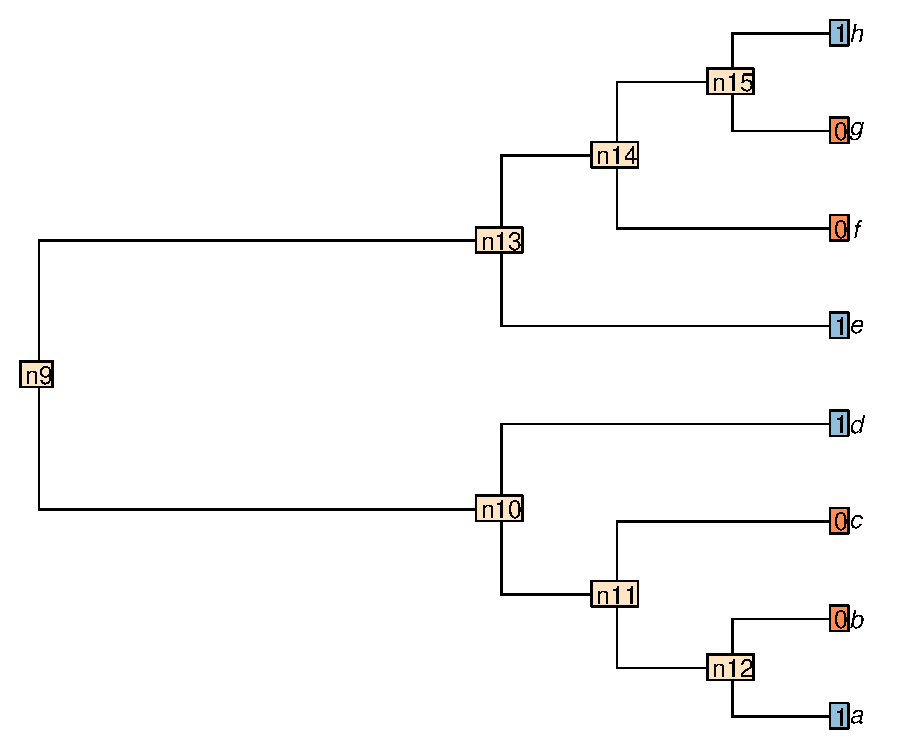
\includegraphics{Inapplicable_data_files/figure-latex/unnamed-chunk-5-1.pdf}

We can use the \texttt{Inapp} package to apply the Fitch algorithm for
this character on this tree.

\begin{Shaded}
\begin{Highlighting}[]
\NormalTok{## Loading the Inapp package}
\KeywordTok{library}\NormalTok{(Inapp)}

\NormalTok{## The tree}
\NormalTok{tree <-}\StringTok{ }\KeywordTok{read.tree}\NormalTok{(}\DataTypeTok{text =} \StringTok{"((((a, b), c), d), (e, (f, (g, h))));"}\NormalTok{)}

\NormalTok{## The character}
\NormalTok{character <-}\StringTok{ "10011001"}

\NormalTok{## Applying the Fitch algorithm}
\NormalTok{matrix <-}\StringTok{ }\KeywordTok{apply.reconstruction}\NormalTok{(tree, character, }\DataTypeTok{method =} \StringTok{"Fitch"}\NormalTok{, }\DataTypeTok{passes =} \DecValTok{2}\NormalTok{)}
\end{Highlighting}
\end{Shaded}

\hypertarget{downpass}{%
\section{Downpass}\label{downpass}}

The downpass is quite simple and follows these rules for the two
possible cases in the traversal:

\begin{enumerate}
\def\labelenumi{\arabic{enumi}.}
\tightlist
\item
  If the two considered tips or nodes have \emph{at least one state in
  common}, set the node to be these states in \emph{common}.
\item
  Else, if there is \emph{nothing in common} between the to tips or
  nodes, set the node to be the \emph{union} of the two states.
\end{enumerate}

For example, node \texttt{n15} is case 2 because there is \emph{nothing
in common} between the tips \texttt{h} and \texttt{g} (states \texttt{1}
and \texttt{0} respectively). Node \texttt{n14} is case 1 because there
is \emph{at least one state in common} between the tip \texttt{f} and
the node \texttt{n15} (state \texttt{0}).

\begin{quote}
Important: when the case 2 is encountered, a transformation is implied
in the descendants of the considered node. The score of the tree is
incremented by +1.
\end{quote}

In the following example, nodes that are in case 1 are in white and
nodes in case 2, which imply a transformation (i.e.~that adds to the
tree score), are in green.

\begin{Shaded}
\begin{Highlighting}[]
\NormalTok{## Plotting the first downpass}
\KeywordTok{plot.states.matrix}\NormalTok{(matrix, }\DataTypeTok{passes =} \DecValTok{1}\NormalTok{, }\DataTypeTok{counts =} \DecValTok{2}\NormalTok{, }\DataTypeTok{show.labels =} \KeywordTok{c}\NormalTok{(}\DecValTok{1}\NormalTok{,}\DecValTok{2}\NormalTok{))}
\KeywordTok{tiplabels}\NormalTok{(char, }\DataTypeTok{cex =} \DecValTok{1}\NormalTok{, }\DataTypeTok{bg =}\NormalTok{ Inapp}\OperatorTok{::}\NormalTok{brewer[[}\DecValTok{2}\NormalTok{]][char }\OperatorTok{+}\StringTok{ }\DecValTok{1}\NormalTok{], }\DataTypeTok{adj =} \DecValTok{1}\NormalTok{)}
\end{Highlighting}
\end{Shaded}

\begin{figure}
\centering
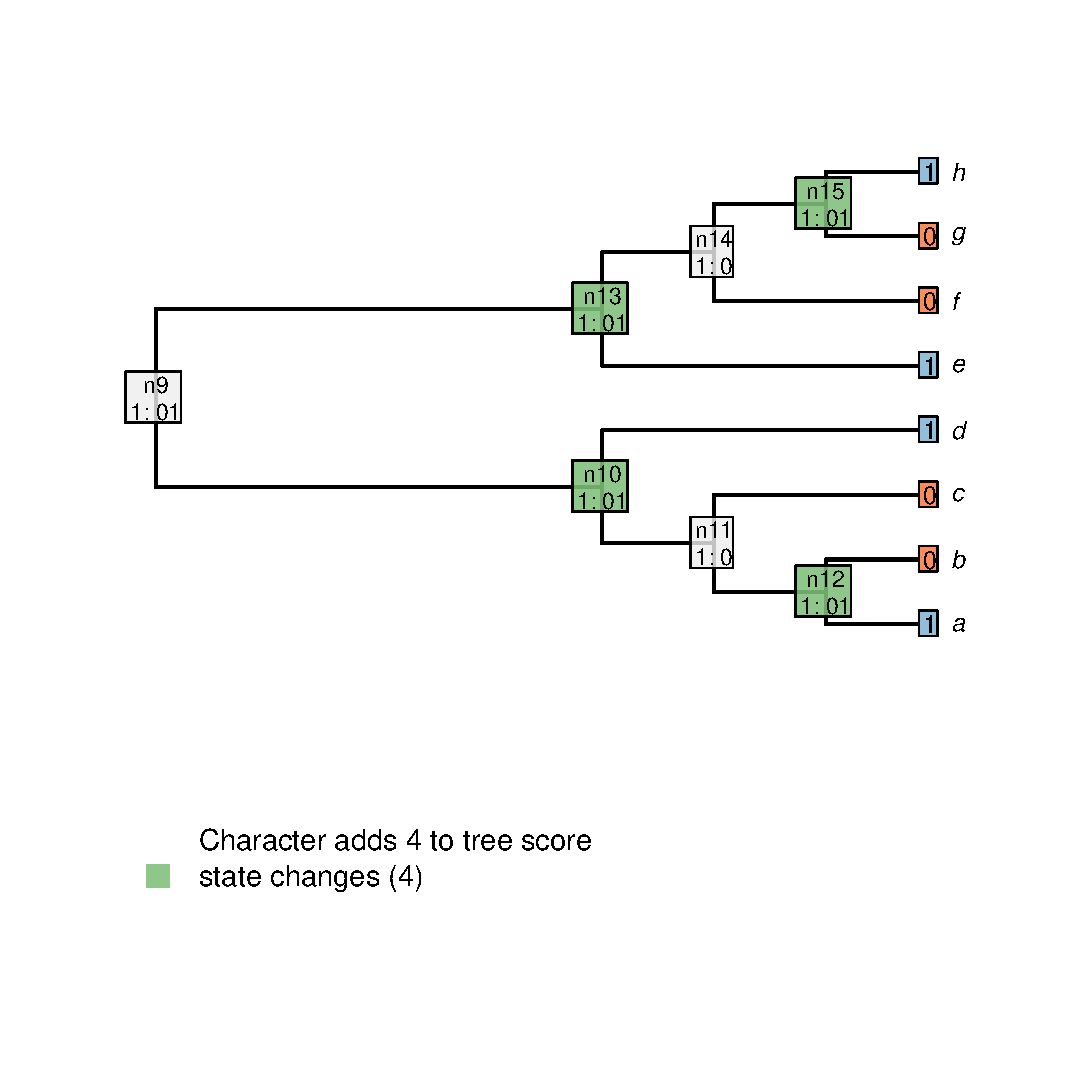
\includegraphics{Inapplicable_data_files/figure-latex/unnamed-chunk-7-1.pdf}
\caption{\label{fig:unnamed-chunk-7}Node reconstructions after downpass}
\end{figure}

\hypertarget{uppass}{%
\section{Uppass}\label{uppass}}

The score of the tree is known after the downpass, but the states of
some nodes might not yet be properly resolved. For example, parsimonious
reconstructions exist that reconstruct node \texttt{n14} as state
\texttt{1}, as opposed to the \texttt{0} presently reconstructed. The
present reconstruction seemingly indicates a change from state 1 to
state 0 in an ancestor of \texttt{n14}, and a subsequent change from
state 0 to state 1 in the ancestor of \texttt{h}, but an alternative
reconstruction is equally parsimonious: \texttt{n13}, \texttt{n14} and
\texttt{n15} may all have state \texttt{1}, with a change from state
\texttt{1} to state \texttt{0} in each of the two lineages leading to
\texttt{f} and \texttt{g}.

The uppass traversal employs the following rules:

\begin{enumerate}
\def\labelenumi{\arabic{enumi}.}
\tightlist
\item
  If the current node and its ancestor have \emph{all states in common},
  the node is already resolved.
\item
  If there is \emph{at least one state in common} between both left and
  right tips or nodes directly descended from the current node, resolve
  the node as being \emph{the states in common} between its ancestor and
  both his descendants.
\item
  If there is \emph{there are no states in common} between its
  descendants, resolve the node as being \emph{the states in common}
  between the ancestor and the current node.
\end{enumerate}

For example, node \texttt{n13} is already resolved (it has all its
states in common with the ancestor - case 1). Node \texttt{n14} has not
all its states in common with its ancestor but its two descendants
(\texttt{n15} and \texttt{f}) have at least one state in common
(\texttt{0}). This node is thus solved to be the states in common
between both descendants (\texttt{01}) and its ancestor (\texttt{01} as
well).

\begin{Shaded}
\begin{Highlighting}[]
\NormalTok{## Plotting the first uppass}
\KeywordTok{plot.states.matrix}\NormalTok{(matrix, }\DataTypeTok{passes =} \DecValTok{1}\OperatorTok{:}\DecValTok{2}\NormalTok{, }\DataTypeTok{counts =} \DecValTok{2}\NormalTok{,}
                   \DataTypeTok{show.labels =} \KeywordTok{c}\NormalTok{(}\DecValTok{1}\NormalTok{, }\DecValTok{2}\NormalTok{), }\DataTypeTok{col.states=}\OtherTok{TRUE}\NormalTok{)}
\end{Highlighting}
\end{Shaded}

\begin{figure}
\centering
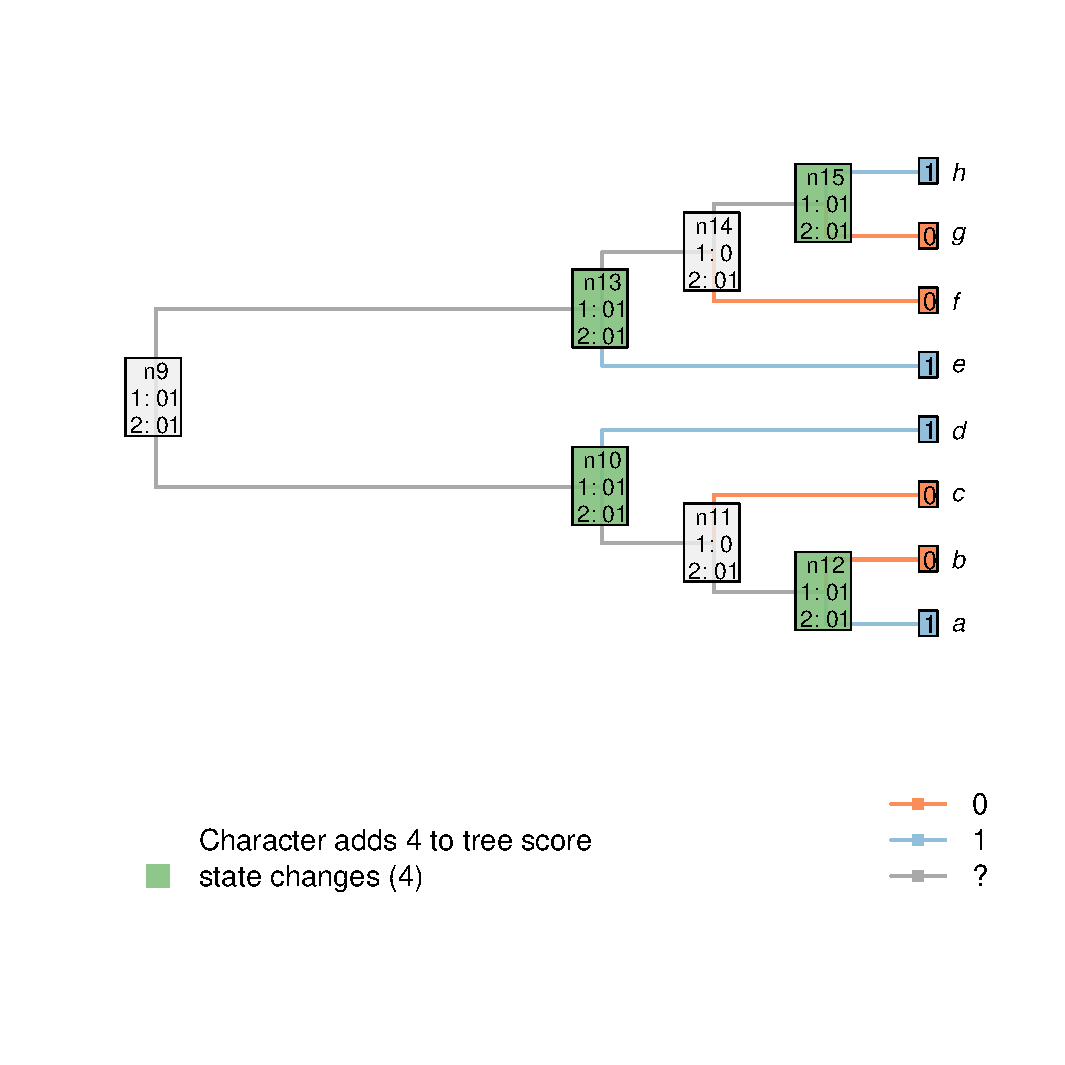
\includegraphics{Inapplicable_data_files/figure-latex/unnamed-chunk-8-1.pdf}
\caption{\label{fig:unnamed-chunk-8}Node reconstructions after uppass}
\end{figure}

More complex cases can be studied in the Inapp App (running in your
favourite web browser) by switching the
\textbf{\texttt{Reconstruction\ method}} to
\textbf{\texttt{Normal\ Fitch}}.

\begin{Shaded}
\begin{Highlighting}[]
\NormalTok{## Running the Inapp App}
\KeywordTok{runInapp}\NormalTok{()}
\end{Highlighting}
\end{Shaded}

\hypertarget{resolving-ambiguous-resolutions}{%
\section{Resolving ambiguous
resolutions}\label{resolving-ambiguous-resolutions}}

In certain cases, it is necessary to go further and discriminate between
the equally-parsimonious reconstructions provided by the Fitch
algorithm. A number of approaches have been proposed concerning which
resolution of ambiguous nodes is preferable.

The two most familiar approaches to resolving ambiguous node are the
Accelerated Transformation (\textsc{AccTran}) and Delayed Transformation
(\textsc{DelTran}) approaches.

The \textsc{AccTran} approach reconstructs transformations as occurring
as close to the root as possible; the \textsc{DelTran}, as far from the
root as possible.

In this case, the ambiguous resolution of the root leaves two options
for the latter:

\begin{figure}
\centering
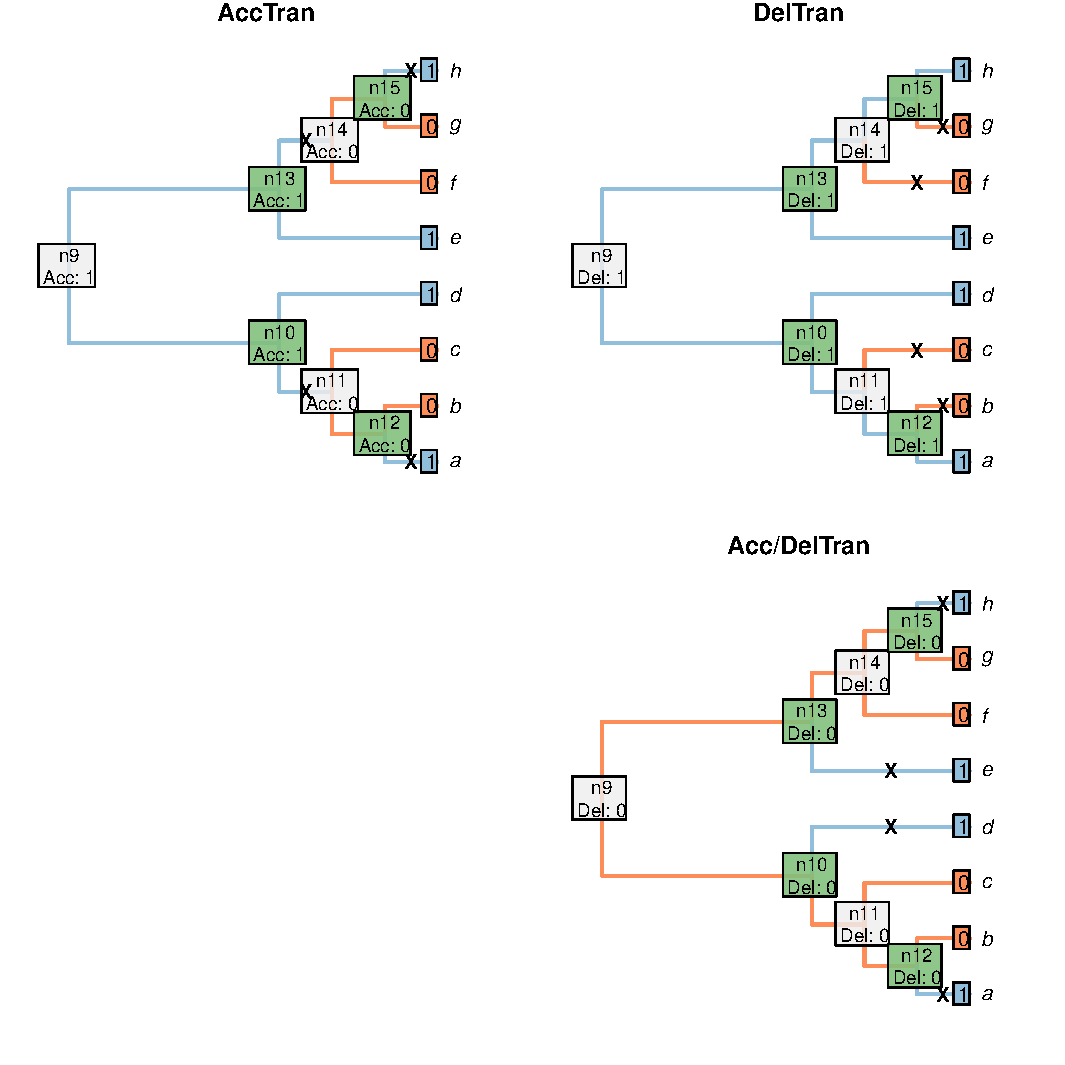
\includegraphics{Inapplicable_data_files/figure-latex/unnamed-chunk-10-1.pdf}
\caption{\label{fig:unnamed-chunk-10}Node reconstructions after AccTran or
DelTran` optimizations}
\end{figure}

If the states \texttt{0} and \texttt{1} represent states of a
transformational character -- whether an organism's tail is red or blue,
say -- then there is no reason to prefer any of the equally-parsimonious
reconstructions, as none implies any more homology than any other.

With neomorphic characters, however, state \texttt{0} stands for the
absence of a character -- for example, a tail -- and state \texttt{1}
its presence. On one view, a reconstruction that minimises the number of
times that such a character evolves attributes more similarity to
homology than an equally parsimonious reconstruction in which said
character is gained multiple times independently.

\hypertarget{maximising-homology}{%
\subsection{Maximising homology}\label{maximising-homology}}

Neither \textsc{AccTran} nor \textsc{DelTran} is guaranteed to maximise
homology \citep{Agnarsson2008}. In this particular case, the
\textsc{DelTran} reconstruction maximises homology. If the character
denotes the presence or absence of a tail, then this reconstruction
invokes the presence of a tail in the common ancestor of all taxa,
meaning that the tails present in tips \texttt{a}, \texttt{d},
\texttt{e} and \texttt{h} are homologous with one another. The
\textsc{AccTran} reconstruction, in contrast, identifies a loss of a
tail at nodes 11 and 14, with a tail evolving independently in tips
\texttt{a} and \texttt{h}. Under this reconstruction, the tails of
\texttt{a} and \texttt{h} are not homologous with each other, or with
the tails of \texttt{d} and \texttt{e}. (The alternative
\textsc{DelTran} approach, which could arguably be described as
\textsc{AccTran} instead, invokes four independent origins of the
character and clearly does not maximise its homology.)

Where we wish to maximise homology, we modify the Fitch uppass such that
any node whose final state reconstruction would be ambiguous is instead
reconstructed as present when that node is encountered. This approach
maximises homology in the problematic trees presented by Agnarsson \&
Miller \citeyearpar{Agnarsson2008}(``A\&M'' below):

\begin{figure}
\centering
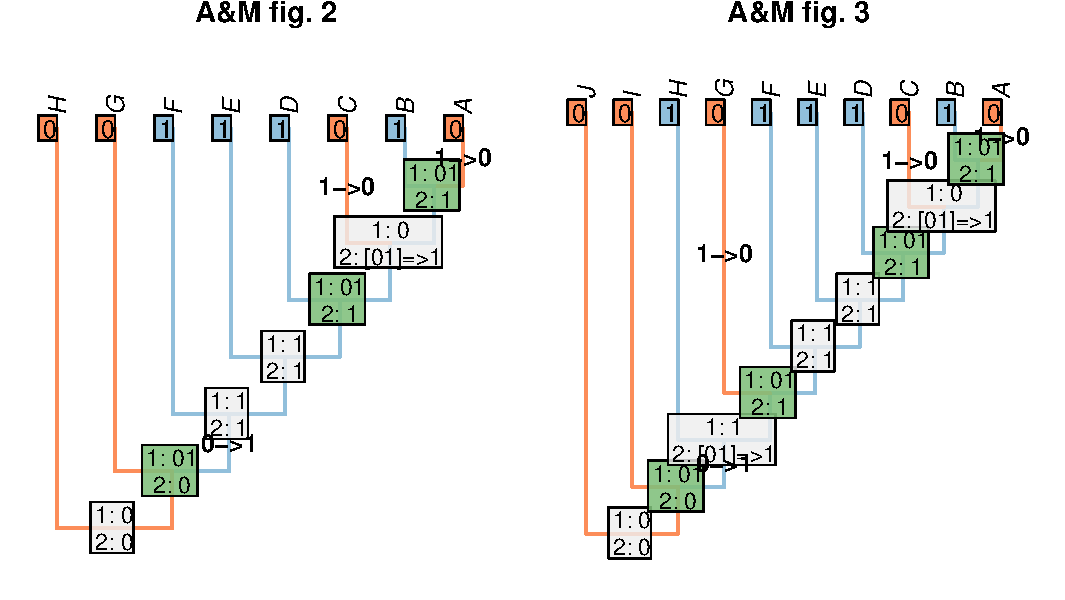
\includegraphics{Inapplicable_data_files/figure-latex/unnamed-chunk-11-1.pdf}
\caption{\label{fig:unnamed-chunk-11}Homology-maximising character
optimisations}
\end{figure}

This approach is also robust to missing entries:

\begin{figure}
\centering
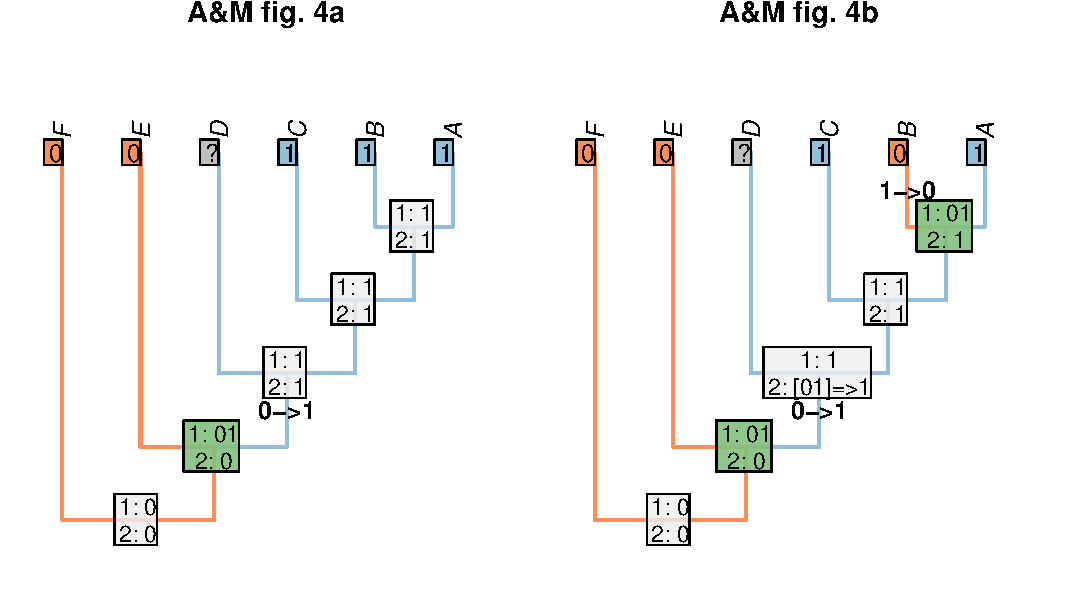
\includegraphics{Inapplicable_data_files/figure-latex/unnamed-chunk-12-1.pdf}
\caption{\label{fig:unnamed-chunk-12}Homology maximisation with missing
entries}
\end{figure}

\hypertarget{problems}{%
\chapter{Problems with the Fitch algorithm}\label{problems}}

The Fitch algorithm counts changes in a character. It assumes that the
character is applicable throughout the tree. This assumption does not
lead to error if:

\begin{itemize}
\item
  The character is inapplicable in fewer than three tips; or
\item
  In the trees being considered, applicable and inapplicable tokens
  occur in distinct regions of the tree \citep{Maddison1993}.
\end{itemize}

\hypertarget{red-tails-blue-tails}{%
\section{Red tails, blue tails}\label{red-tails-blue-tails}}

Maddison \citeyearpar{Maddison1993} provided the following example to
demonstrate the problem encountered by the Fitch algorithm when
inapplicable characters were present.

Consider the following tree, each node of which is supported by a number
of characters. Tail colour (illustrated; 0 = red, 1 = blue) has not yet
been considered, but has the potential to resolve the polytomy on the
left hand side (bold).

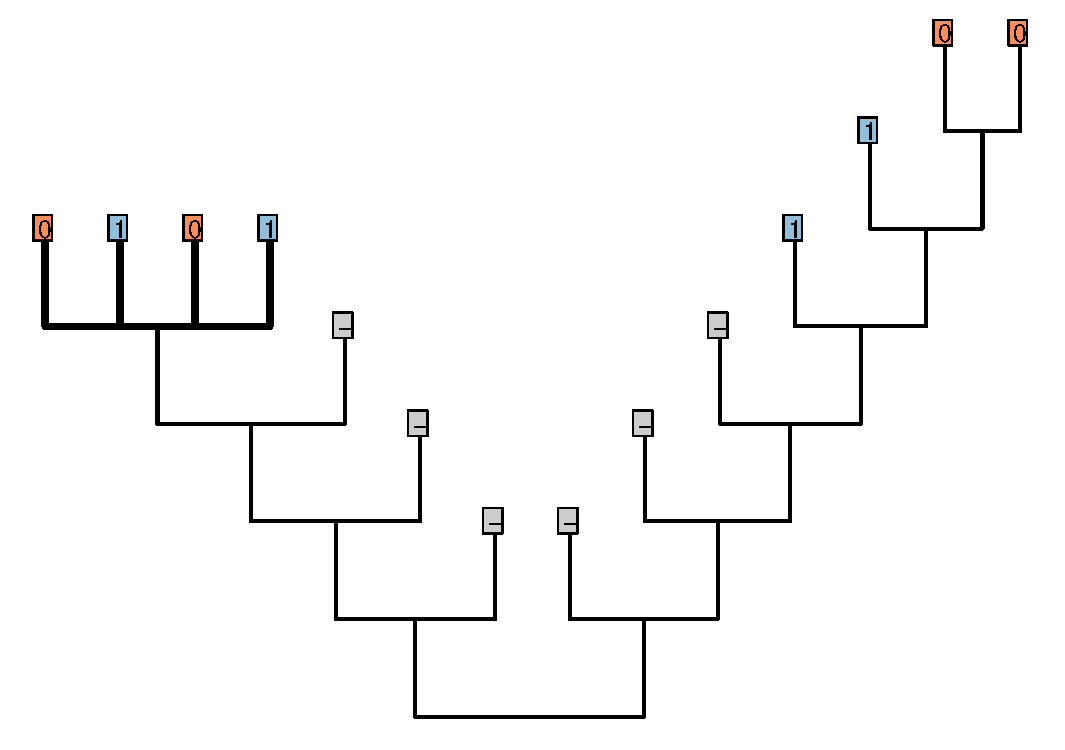
\includegraphics{Inapplicable_data_files/figure-latex/unnamed-chunk-14-1.pdf}

In the bold region, tail colour should group the red-tailed tips
together, and the blue-tailed tips together, but does not establish
whether the ancestor of the left-hand tail-bearing clade had a red or
blue tail.

\begin{figure}
\centering
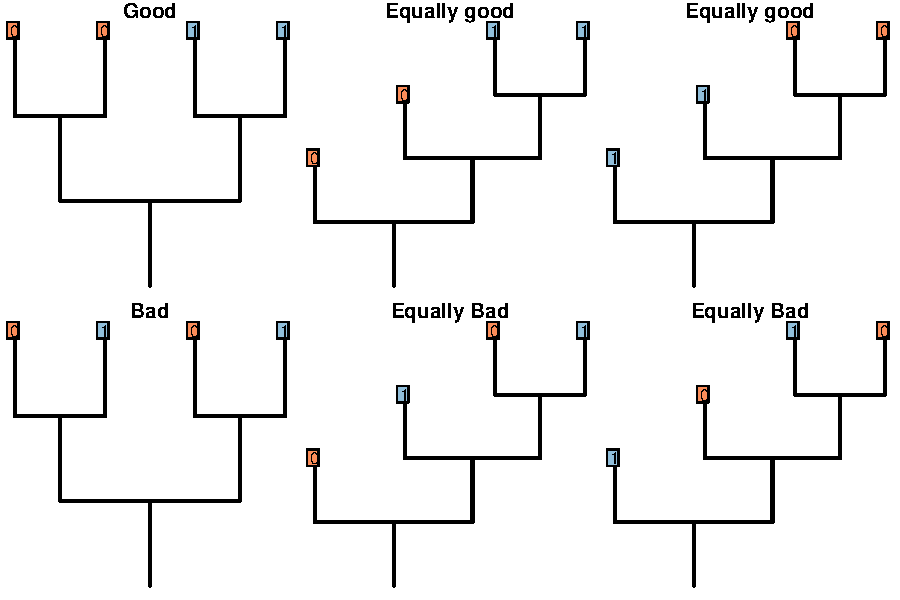
\includegraphics{Inapplicable_data_files/figure-latex/unnamed-chunk-15-1.pdf}
\caption{\label{fig:unnamed-chunk-15}Possible resolutions for bold region of
tree (Good ones imply only one change)}
\end{figure}

\hypertarget{reductive-coding}{%
\section{Reductive coding}\label{reductive-coding}}

Under reductive coding, the tail and its colour are described in two
character statements:

\begin{quote}
Tail: (0), absent; (1), present.

Tail, colour: (0), red; (1), blue; (?), inapplicable.
\end{quote}

Consider the following two trees, each of which receives a score of two
for the first character (presence of tail). The score of the second
character (tail colour) is not as desired.

The Fitch algorithm will prefer trees in which the left-hand
tail-bearing clade has a blue tail, simply because the right-hand
tail-bearing clade ancestrally did.

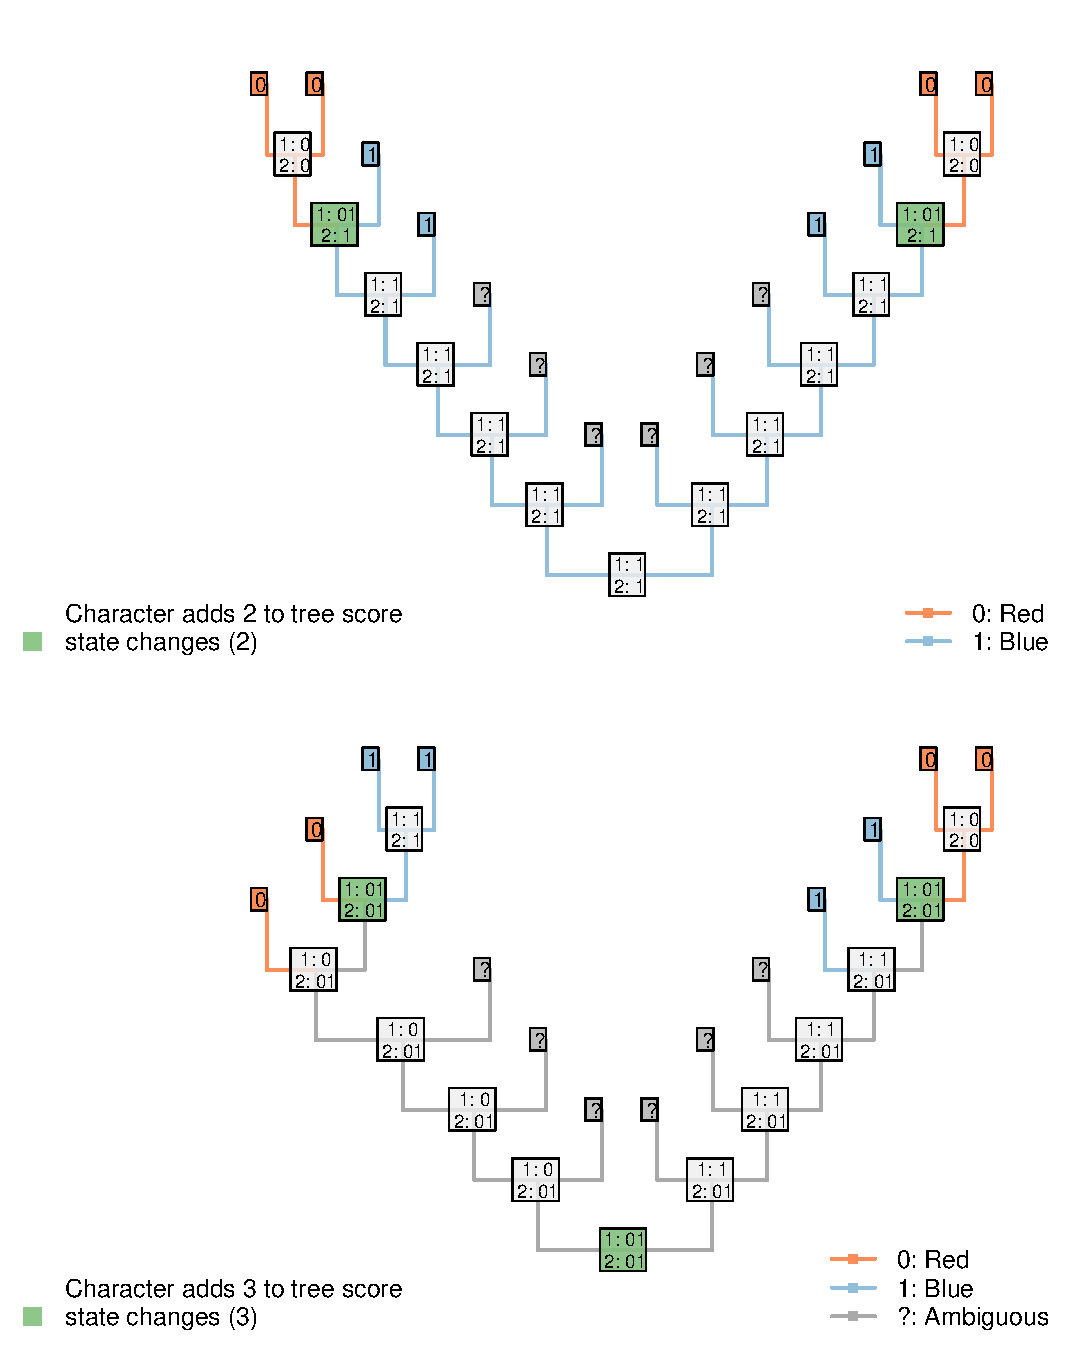
\includegraphics{Inapplicable_data_files/figure-latex/unnamed-chunk-16-1.pdf}

Notice the additional step reconstructed at the root node: the Fitch
algorithm reconstructs a change in tail colour in a taxon that doesn't
have a tail!

This reconstruction is not logically consistent.

\hypertarget{an-exception}{%
\subsection{An exception}\label{an-exception}}

If the parent character can parsimoniously be reconstructed as present
at every internal node in a single unbroken region of a tree, and
nowhere else, then reductive coding does work successfully. Reductive
coding may therefore be appropriate if only a subset of all possible
trees are under consideration, and is always (i.e.~for all trees)
appropriate if a character exhibits fewer than three inapplicable
tokens.

\hypertarget{inapplicable-as-an-extra-state}{%
\section{Inapplicable as an extra
state}\label{inapplicable-as-an-extra-state}}

An alternative is to code the inapplicable token as an extra state:

\begin{quote}
Tail: (0), absent; (1), present.

Tail, colour: (0), red; (1), blue; (2), inapplicable.
\end{quote}

This seems to resolve the problem case that we encountered with
reductive coding:

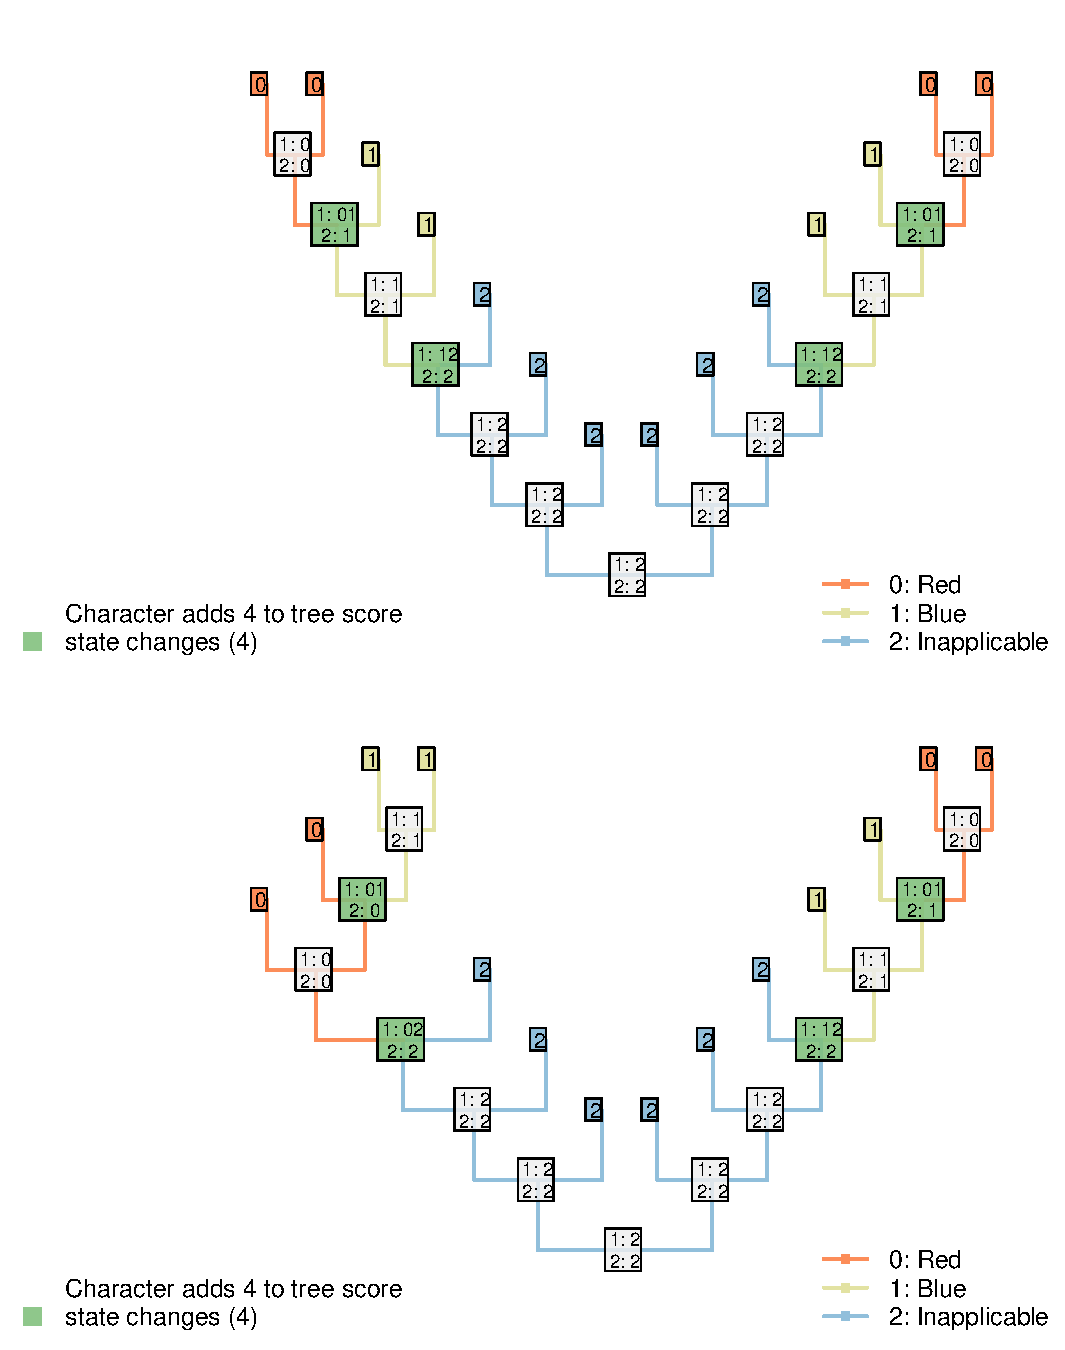
\includegraphics{Inapplicable_data_files/figure-latex/unnamed-chunk-17-1.pdf}

Both trees now receive the same score for the `tail colour' character,
which contributes four steps. Two of these steps, however, correspond to
steps that have already been counted in the parent character, reflecting
the two gains of a tail.

Although this reconstruction is logically consistent, the gain (or loss)
of the tail is now reflected in two characters -- characters are not
independent of one another.

The outcome is that each ontologically dependent character serves to
increase the weight of its parent character. The loss of a tail, for
example, would incur a cost of one step in the tail character and one
step in each ontologically dependent character, even though it
represents a single evolutionary event.

\hypertarget{a-single-multi-state-character}{%
\section{A single multi-state
character}\label{a-single-multi-state-character}}

A different approach is to use a single character to denote both the
presence and the colour of the tail:

\begin{quote}
Tail: (0), absent; (1), present, red; (2), present, blue.
\end{quote}

This seems to resolve the problem case that we encountered with
reductive coding:

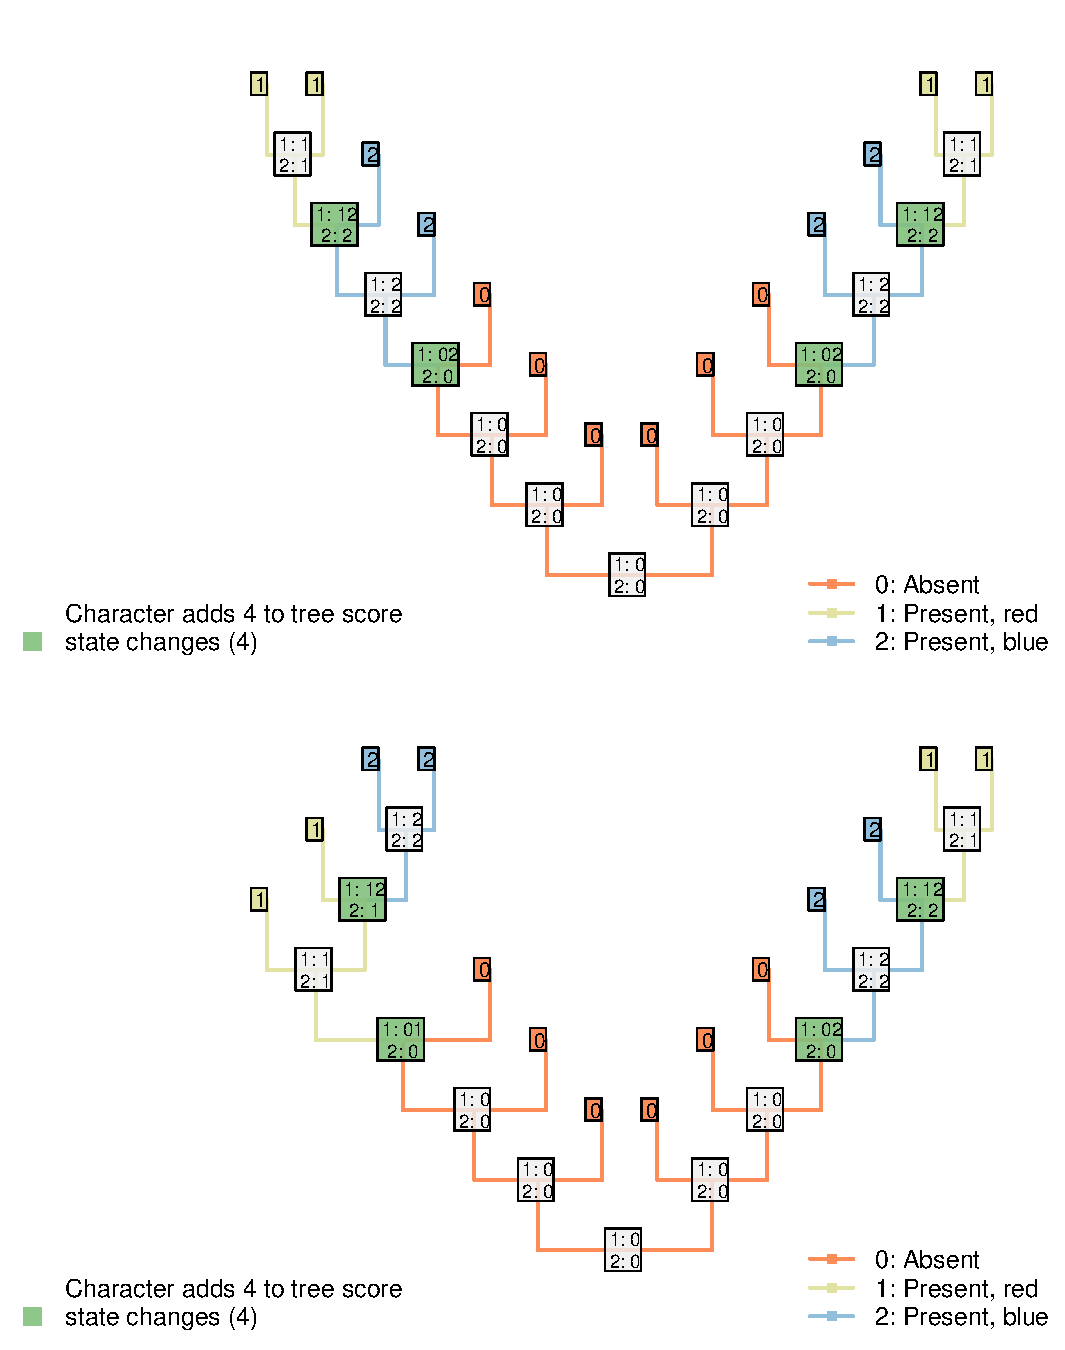
\includegraphics{Inapplicable_data_files/figure-latex/unnamed-chunk-18-1.pdf}

However, we now have a situation where the gain/loss of a tail is
afforded the same weight as a change in tail colour. We ought to prefer
a tree where the tail evolved once (and changed colour) to one where it
evolved twice (being a different colour each time).

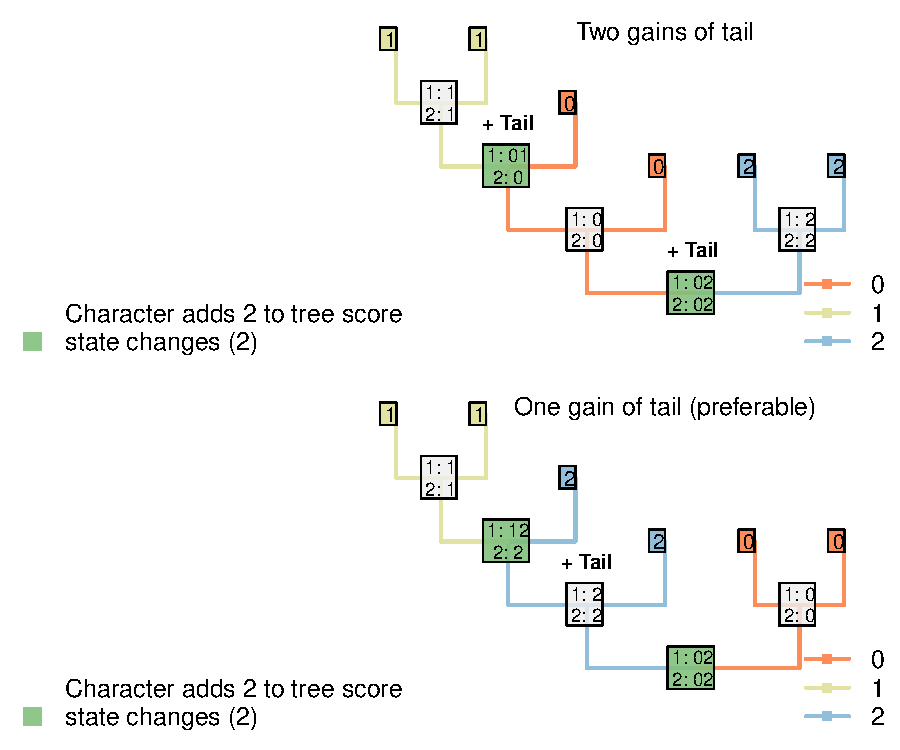
\includegraphics{Inapplicable_data_files/figure-latex/unnamed-chunk-19-1.pdf}

\hypertarget{sankoff-matrices}{%
\section{Sankoff matrices}\label{sankoff-matrices}}

It would be possible to establish a Sankoff matrix such that a change
between absent and red or absent and blue cost more than a change
between red and blue, but this effectively up-weights the tail
character, and it's not clear that this is desirable -- or how much this
extra weight should be \citep{Maddison1993}.

\hypertarget{symmetric}{%
\subsection{Symmetric}\label{symmetric}}

Consider a character with three ontologically dependent characters:

\begin{quote}
Presence: Absent / present

Colour: Red / blue

Covering: Scaly / hairy

Shape: Straight / curly
\end{quote}

This could be coded as a single transformation series using a Sankoff
matrix:

\begin{table}

\caption{\label{tab:unnamed-chunk-20}Tail: Cost to go from left state to top state:}
\centering
\begin{tabular}[t]{l|l|l|l|l|l|l|l|l}
\hline
  & 0 & 1 & 2 & 3 & . & . & . & 8\\
\hline
(0), absent & 0 & 4 & 4 & 4 & . & . & . & 4\\
\hline
(1), present, red, scaly, straight & 4 & 0 & 1 & 1 & . & . & . & 3\\
\hline
(2), present, red, scaly, curly & 4 & 1 & 0 & 2 & . & . & . & 2\\
\hline
(3), present, red, hairy, straight & 4 & 1 & 2 & 0 & . & . & . & 2\\
\hline
. & . & . & . & . & 0 & . & . & .\\
\hline
. & . & . & . & . & . & 0 & . & .\\
\hline
. & . & . & . & . & . & . & 0 & .\\
\hline
(8), present, blue, hairy, curly & 4 & 3 & 2 & 2 & . & . & . & 0\\
\hline
\end{tabular}
\end{table}

The first thing to note is that each additional ontologically depedent
character generates disproportionately more complexity in the Sankoff
matrix.

Even if this additional complexity could be handled, the underlying
issue remains that losing a tail, which arguably corresponds to a single
evolutionary event, is allocated a large cost (here, 4) that grows in
line with the number of ontogenetically dependant characters.

\hypertarget{gain-and-loss-asymmetric}{%
\subsection{Gain and loss asymmetric}\label{gain-and-loss-asymmetric}}

At the cost of symmetry, one could argue that the loss of a tail
requires a single transformation, whereas the gain requires the addition
of a tail and the ``setting'' of each ontologically dependent character,
rendering an asymmetric Sankoff matrix that nevertheless respects
triangular inequality:

\begin{table}

\caption{\label{tab:unnamed-chunk-21}Tail: Cost to go from left state to top state:}
\centering
\begin{tabular}[t]{l|l|l|l|l|l|l|l|l}
\hline
  & (0) & (1) & (2) & (3) & . & . & . & (8)\\
\hline
(0), absent & 0 & 4 & 4 & 4 & . & . & . & 4\\
\hline
(1), present, red, scaly, straight & 1 & 0 & 1 & 1 & . & . & . & 3\\
\hline
(2), present, red, scaly, curly & 1 & 1 & 0 & 2 & . & . & . & 2\\
\hline
(3), present, red, hairy, straight & 1 & 1 & 2 & 0 & . & . & . & 2\\
\hline
. & . & . & . & . & 0 & . & . & .\\
\hline
. & . & . & . & . & . & 0 & . & .\\
\hline
. & . & . & . & . & . & . & 0 & .\\
\hline
(8), present, blue, hairy, curly & 1 & 3 & 2 & 2 & . & . & . & 0\\
\hline
\end{tabular}
\end{table}

Here, though, we encounter a new problem: reconstructions involving very
many losses are preferred to those involving a single gain.

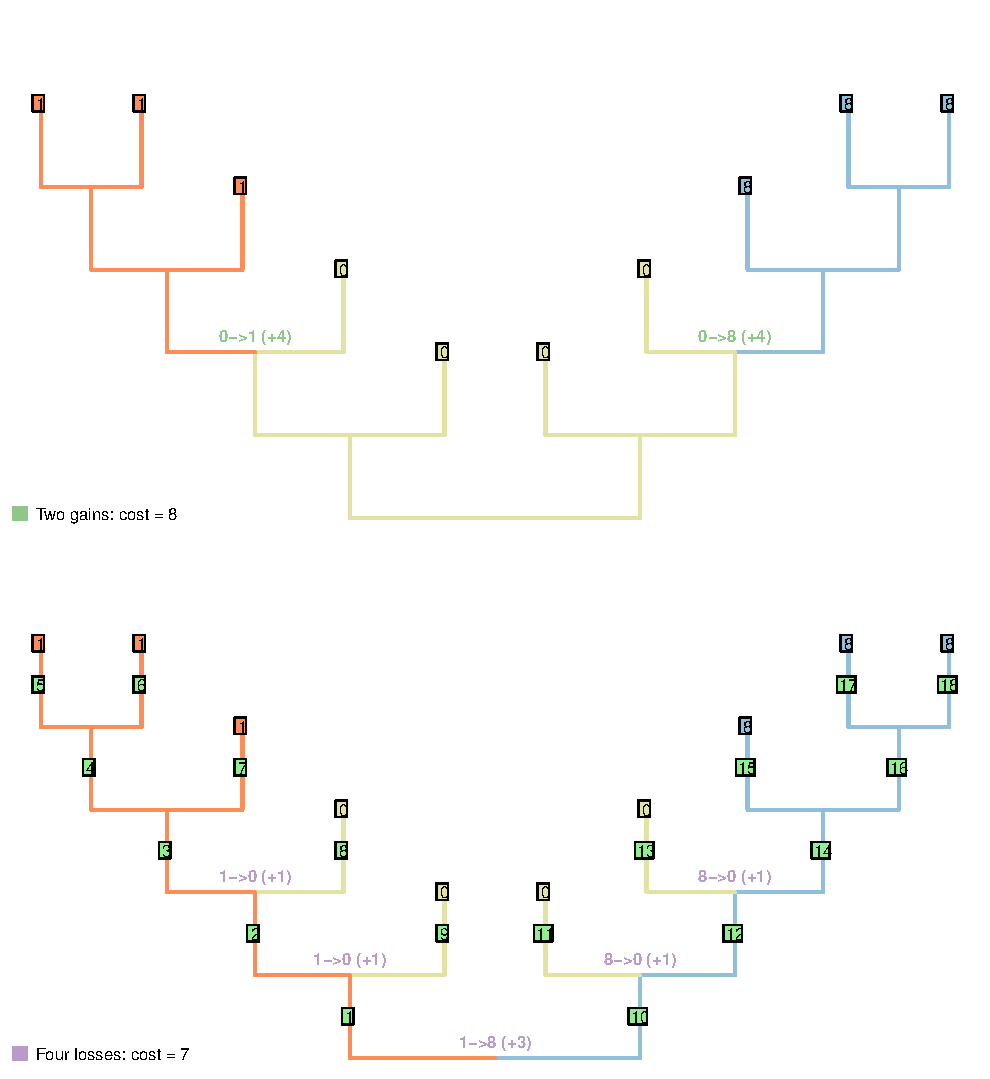
\includegraphics{Inapplicable_data_files/figure-latex/unnamed-chunk-22-1.pdf}

\hypertarget{why-counting-steps-cannot-work}{%
\section{Why counting steps cannot
work}\label{why-counting-steps-cannot-work}}

The failure of the Sankoff approach illustrates a more general problem:
if the only thing that is counted is the number of steps, then trees
that imply multiple gains and losses of a principal character are not
adequately penalised.

To illustrate this point, consider counting only transitions between
applicable states (i.e.~steps), but not transitions from the applicable
state to the inapplicable state:

\begin{figure}
\centering
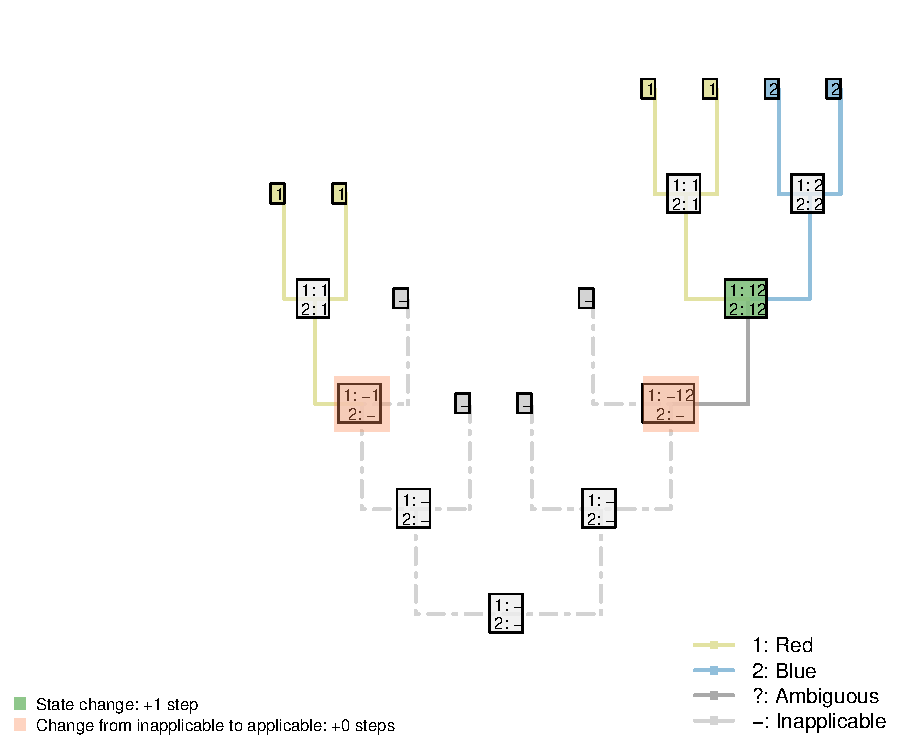
\includegraphics{Inapplicable_data_files/figure-latex/unnamed-chunk-23-1.pdf}
\caption{\label{fig:unnamed-chunk-23}Tail colour optimization}
\end{figure}

The number of steps can be minimized by maximizing the number of
independent gains of a parent character.

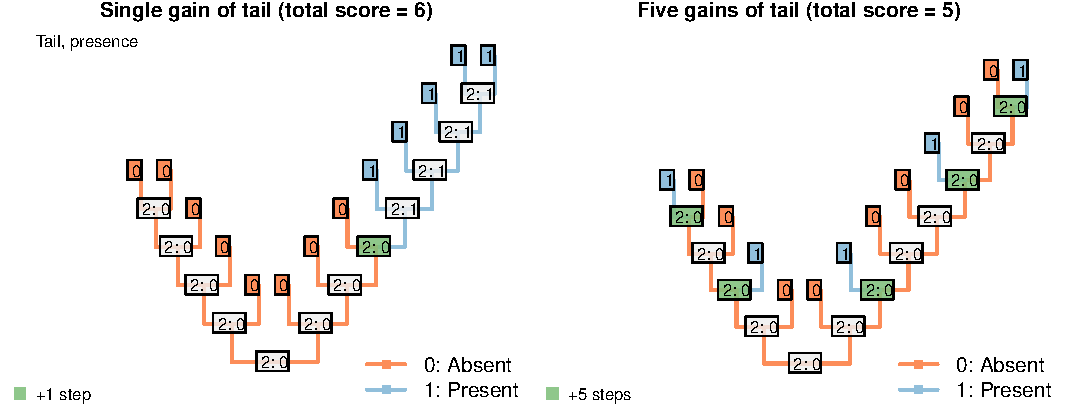
\includegraphics{Inapplicable_data_files/figure-latex/unnamed-chunk-24-1.pdf}
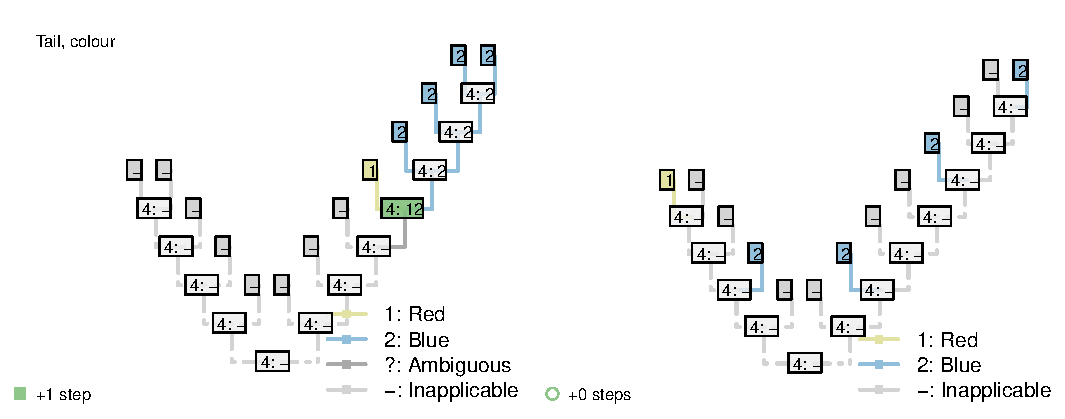
\includegraphics{Inapplicable_data_files/figure-latex/unnamed-chunk-24-2.pdf}
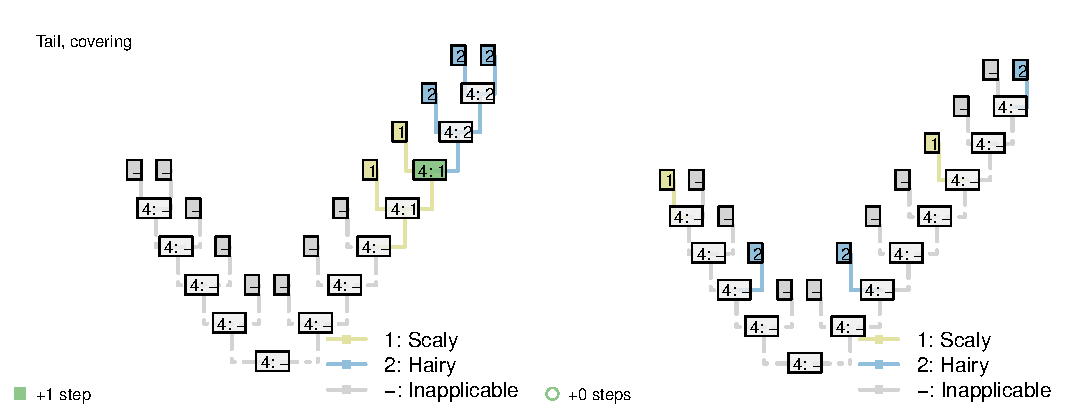
\includegraphics{Inapplicable_data_files/figure-latex/unnamed-chunk-24-3.pdf}
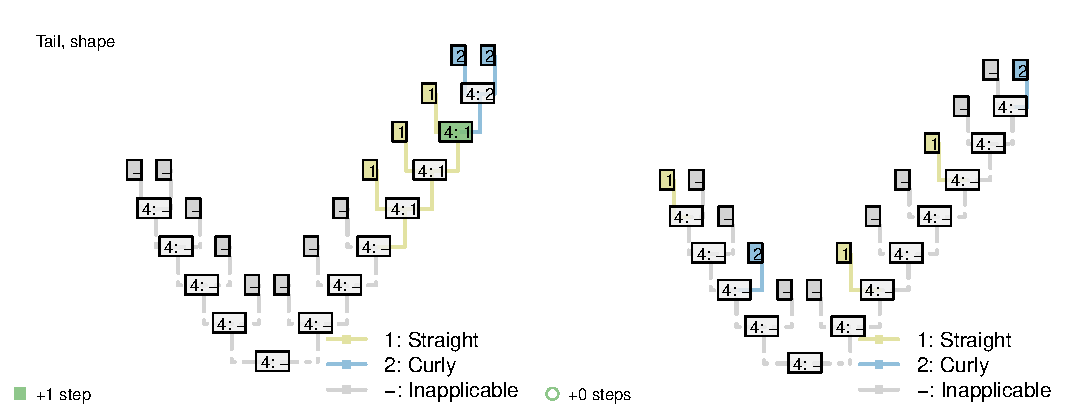
\includegraphics{Inapplicable_data_files/figure-latex/unnamed-chunk-24-4.pdf}
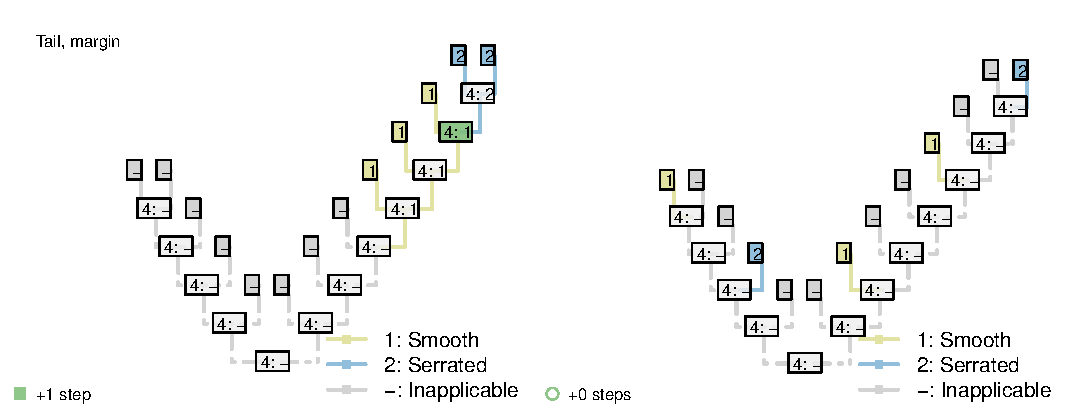
\includegraphics{Inapplicable_data_files/figure-latex/unnamed-chunk-24-5.pdf}
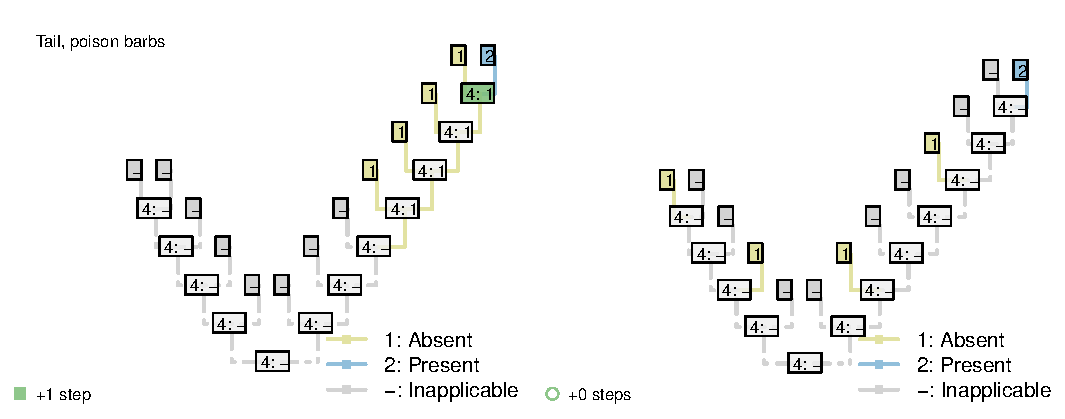
\includegraphics{Inapplicable_data_files/figure-latex/unnamed-chunk-24-6.pdf}

\hypertarget{conclusion}{%
\section{Conclusion}\label{conclusion}}

No coding mechanism can generate consistent and logically meaningful
tree scores when employing the Fitch algorithm. A new algorithm is
needed: one that counts homoplasies instead of steps.

\hypertarget{solution}{%
\chapter{A solution}\label{solution}}

\hypertarget{minimising-homoplasy}{%
\section{Minimising homoplasy}\label{minimising-homoplasy}}

A solution can be found if the goal of parsimony is recast not in terms
of minimising the number of steps, but instead of minimising the amount
of homoplasy in a tree.

De Laet has made this point before
\citetext{\citealp{DeLaet2005}; \citeyear{DeLaet2015}}, suggesting that
a tree's score should be calculated as

\begin{quote}
Total score = Number of steps + Number of (additional) regions.
\end{quote}

Practically, because the number of unavoidable regions is a function of
a dataset and not of a tree, one could alternatively count

\begin{quote}
Total score = Number of steps + Number of regions
\end{quote}

which would be a constant number larger than the total score generated
just counting additional regions; the absolute value of the score is not
meaningful in itself and is not comparable between datasets, so the
calculation method does not affect tree search.

The tree below gives an example of a tree in which a character in
applicable in two regions (one more than the minimum possible, one) and
one state change.

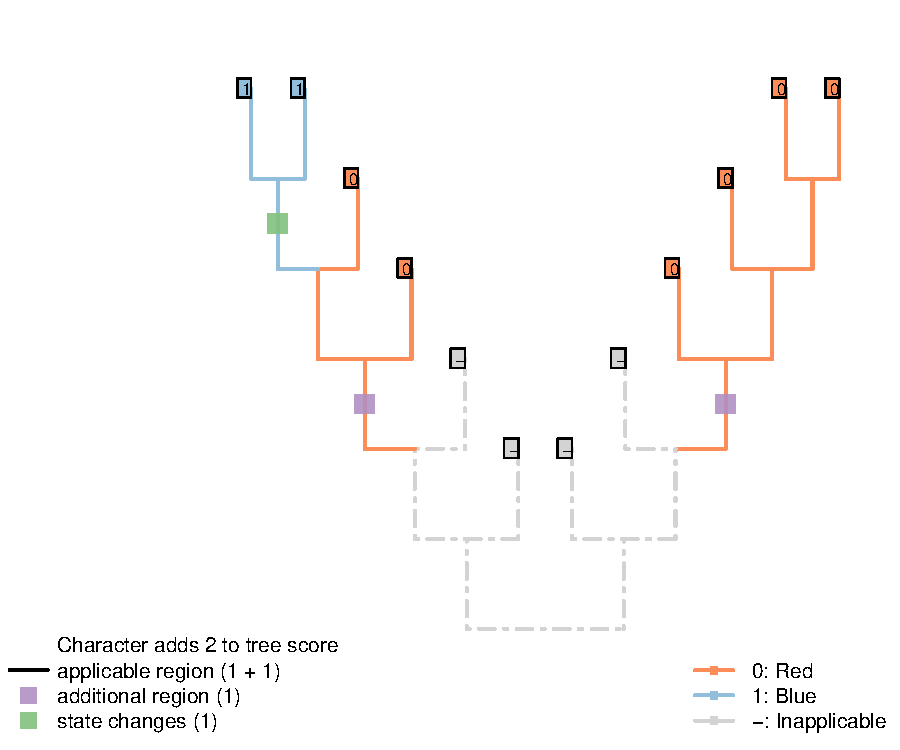
\includegraphics{Inapplicable_data_files/figure-latex/unnamed-chunk-26-1.pdf}

This score denotes two evolutionary observations that cannot be
attributed to inheritance from a common ancestor: the blueness of tail
in the blue tailed taxa (as the common ancestor inherited a red tail),
and the redness of tail in the second region of the tree (as the common
ancestor of all tail-bearing taxa did not itself have a tail, so tail
colour could no be inherited).

\hypertarget{what-does-it-take-to-denote-separate-regions}{%
\subsection{What does it take to denote separate
regions?}\label{what-does-it-take-to-denote-separate-regions}}

It takes three inapplicable nodes (including tips) to force two regions
of the tree to be separrated by an inapplicable region.

This can be estabilshed by imagining the Fitch optimisation of a
separate character

\begin{quote}
Applicability of the character of interest: (0), inapplicable; (1),
applicable
\end{quote}

In the case of tail colour, this applicability character has the same
distribution as the presence / absence of the tail, but this is not
necessarily the case (there may be a range of reasons to code a
character as inapplicable).

In the tree shown above, the Fitch algorithm identifies two regions
where the applicability character is unambiguously `applicable':

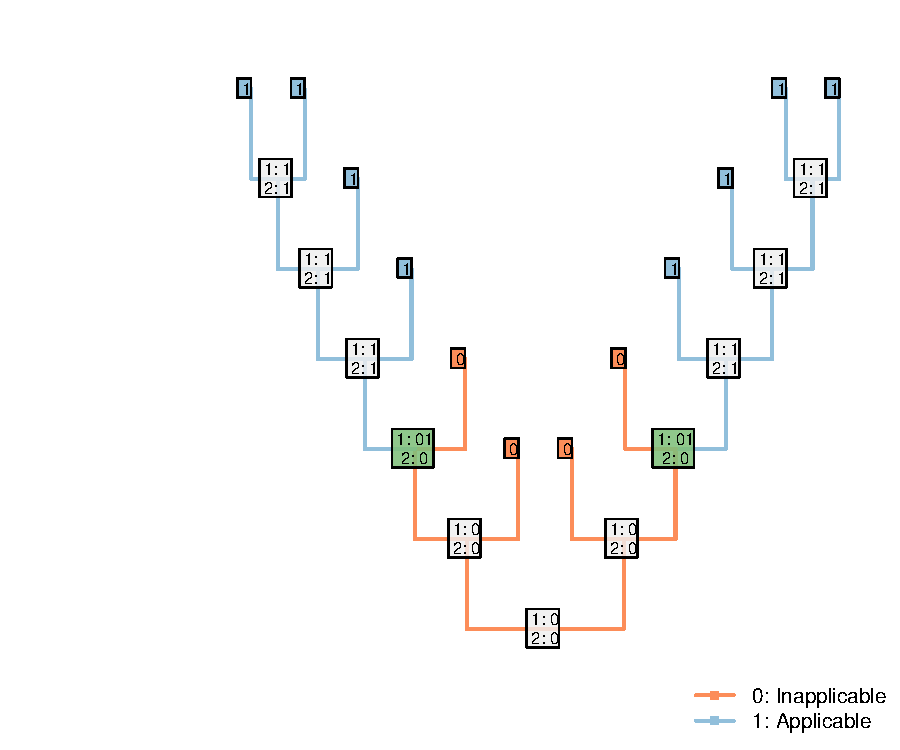
\includegraphics{Inapplicable_data_files/figure-latex/unnamed-chunk-27-1.pdf}

If one of the inapplicable tips had instead been ambiguous, then the
same distribution would arise:

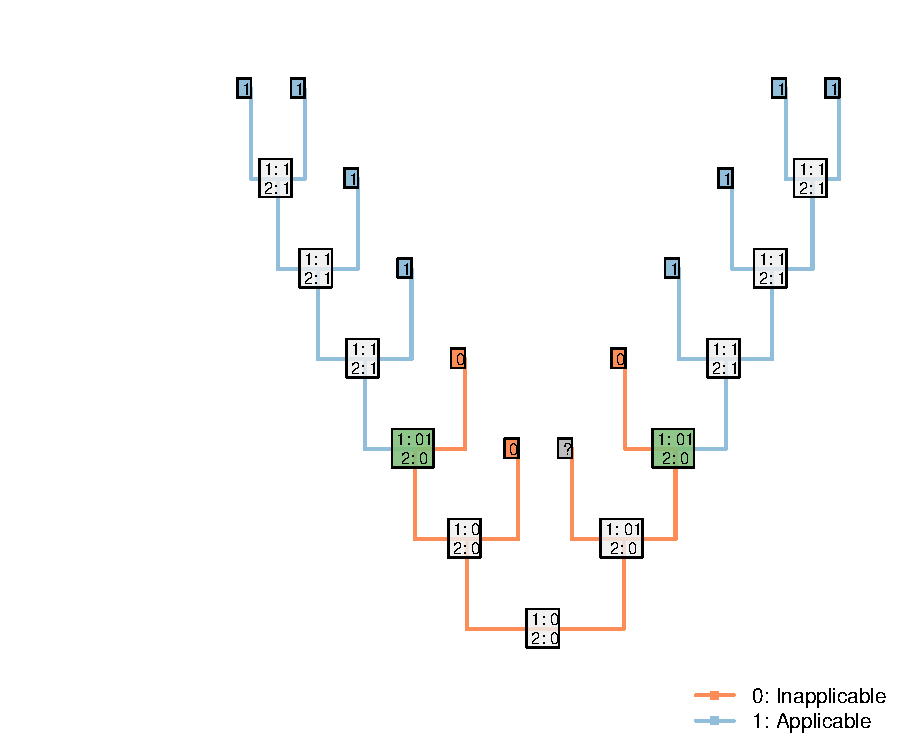
\includegraphics{Inapplicable_data_files/figure-latex/unnamed-chunk-28-1.pdf}

But if two were ambiguous, then the root of the tree could be
parsimoniously reconstructed as `applicable' -- with the two
inapplicable tips becoming inapplicable in the branches that led to
them:

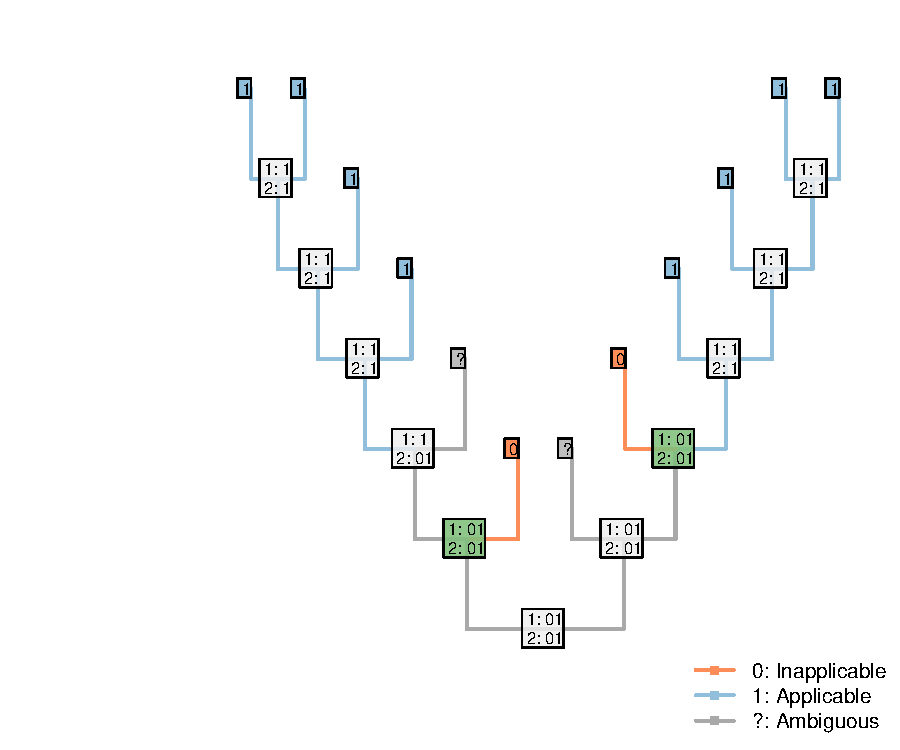
\includegraphics{Inapplicable_data_files/figure-latex/unnamed-chunk-29-1.pdf}

This reconstruction maximises the inferred homology between tails, and
so increases the opportunity to attribute shared colours in the tail to
common ancestry. As such, our algorithm chooses to interpret this region
as applicable whereever it parsimoniously can.

Note that the three inapplicable tips necessary to define an
inapplicable region must be in a contiguous region of the tree,
separated from one another only by taxa whose applicability is
ambiguous, in order for two applicable regions to be reconstructed as
separate.

\hypertarget{how-this-fixes-the-problem}{%
\subsection{How this fixes the
problem}\label{how-this-fixes-the-problem}}

This overcomes the problem where steps could be avoided by inferring
multiple innovations of a character:

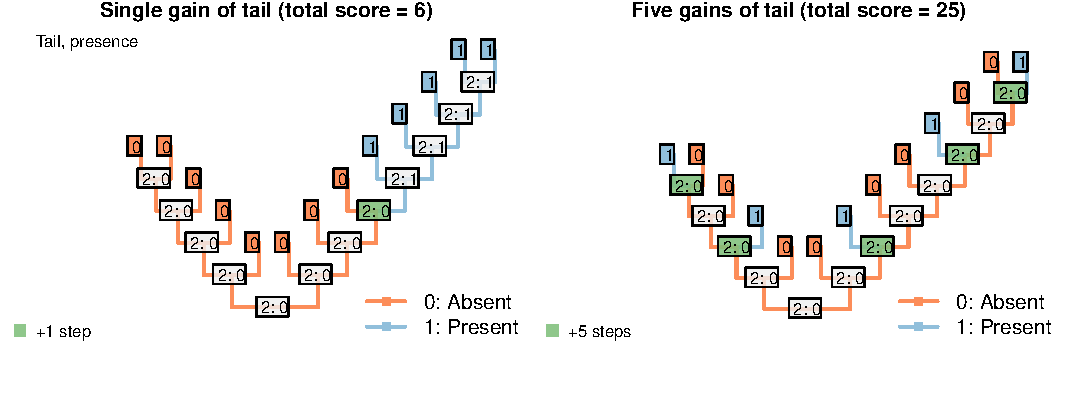
\includegraphics{Inapplicable_data_files/figure-latex/unnamed-chunk-30-1.pdf}
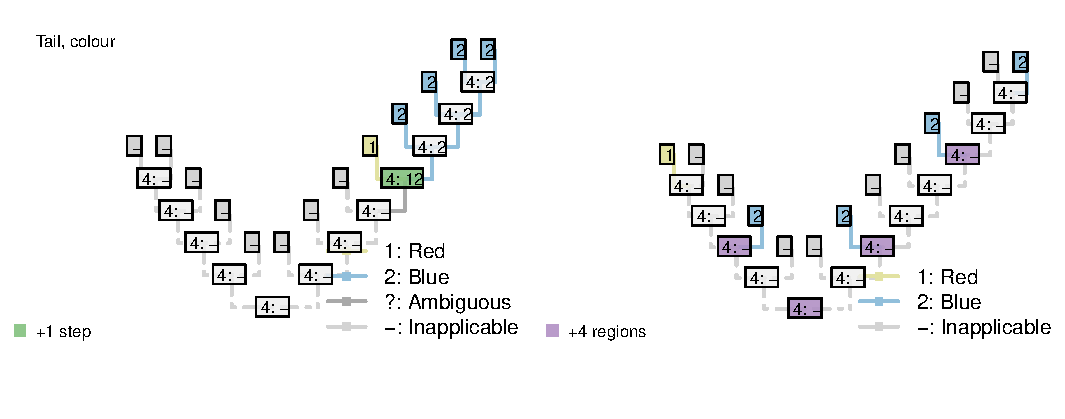
\includegraphics{Inapplicable_data_files/figure-latex/unnamed-chunk-30-2.pdf}
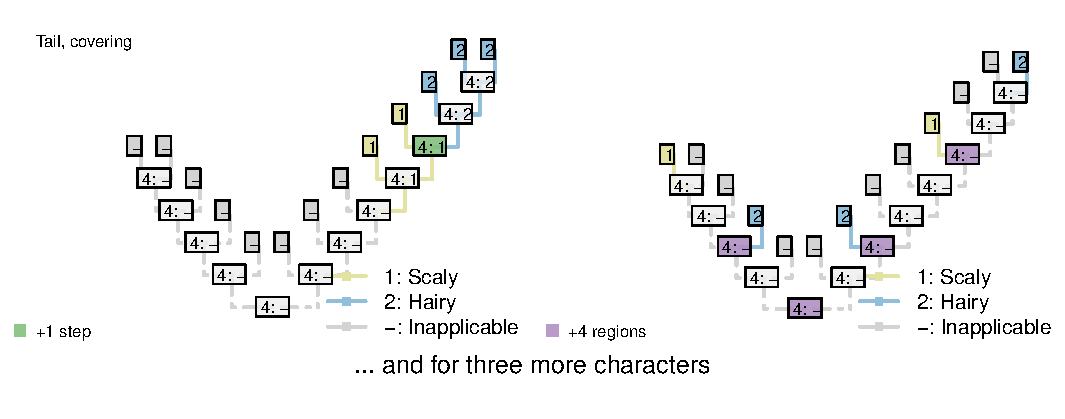
\includegraphics{Inapplicable_data_files/figure-latex/unnamed-chunk-30-3.pdf}

On the other hand, if taxa either have a blue, scaly, straight tail or a
red, smooth, curly tail, then the fact that the tails have so little in
common means that it wouldn't be entirely surprising if the two
different tail types evolved twice. This scenario thus incurs a cost of
only one step (for the additional origin of the tail) more than if the
tail evolved once, and change all its attributes:

\begin{figure}
\centering
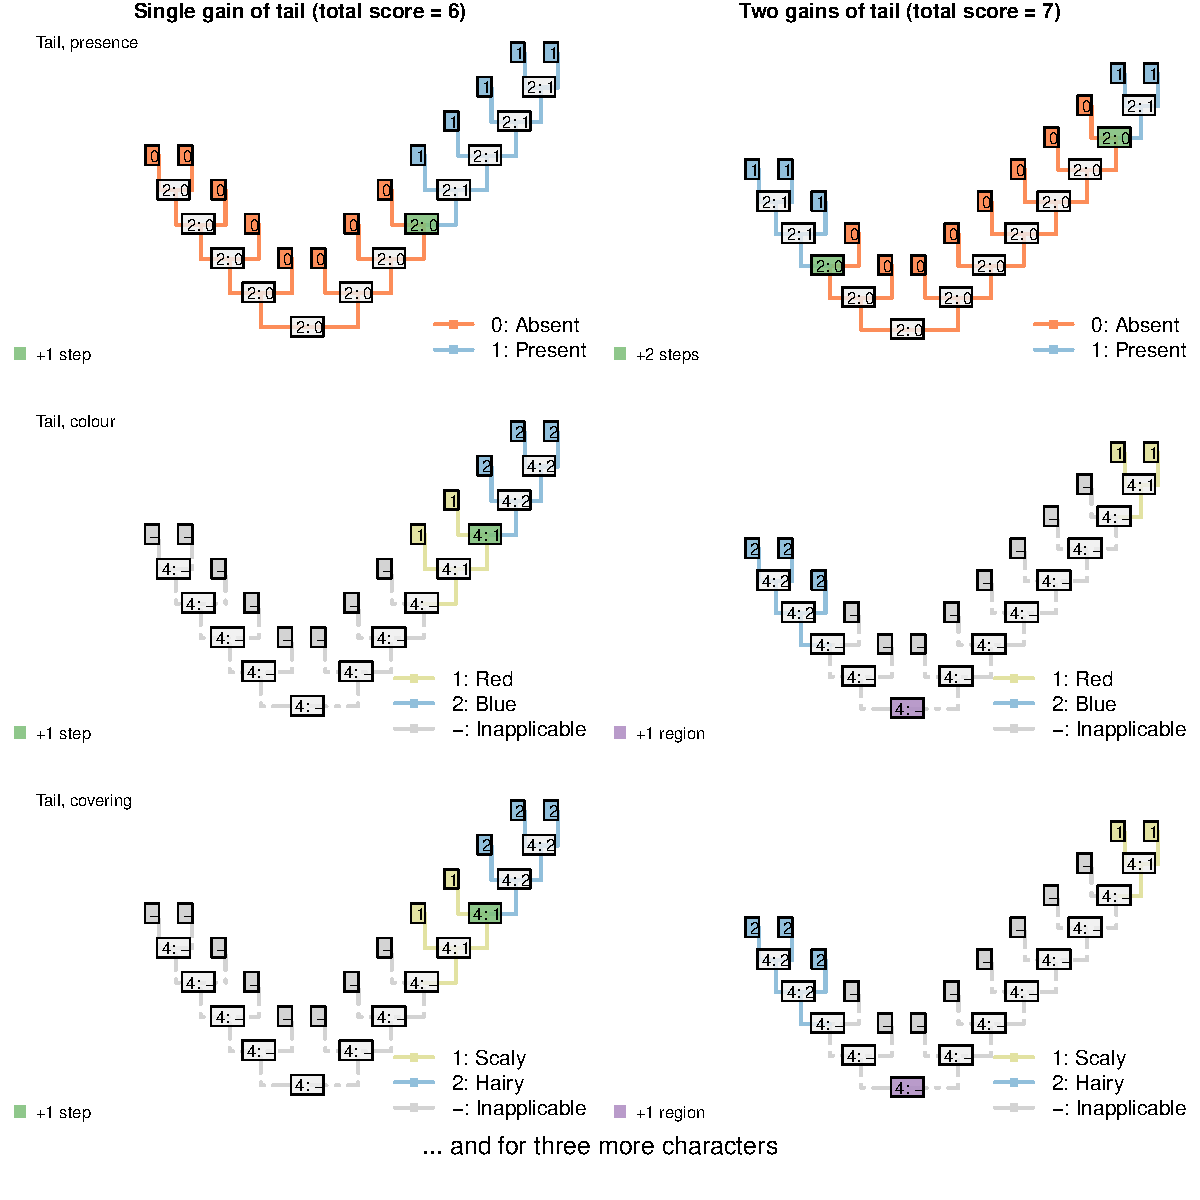
\includegraphics{Inapplicable_data_files/figure-latex/unnamed-chunk-31-1.pdf}
\caption{\label{fig:unnamed-chunk-31}Reconstructions of tail presence and
five contingent characters (only two shown)}
\end{figure}

\hypertarget{summary}{%
\subsection{Summary}\label{summary}}

This is the desired behaviour. But how do we count this in practice?

In brief, we evaluate for each tip whether the character in question is
applicable, inapplicable, or ambiguous (could be either), and use the
standard Fitch algorithm on this applicability data to reconstruct the
state of each internal node, reconstructing ambiguous nodes on the
uppass as applicable.

This done, we conduct a second Fitch-like pass on the tree, in which we
count transformations if they occur at nodes in which the character has
been reconstructed as applicable. Additional regions are also counted on
this downpass, by counting nodes that are ancestral to an inapplicable
region of the tree that itself leads to an as-yet-uncounted applicable
region.

\hypertarget{algorithm}{%
\section{Algorithmic implementation}\label{algorithm}}

Consider a tree with 12 taxa and the following multi-state characters
with inapplicable data \texttt{23-\/-1??-\/-032}; say the character is
``colour of the tail'' ranging from 0 to 3 (four colours). Four taxa in
our example have no tail (hence the inapplicable data \texttt{-}) and
for two taxa, the data is missing (\texttt{?}- we don't known the colour
of the tail or even whether the taxa have a tail or not).

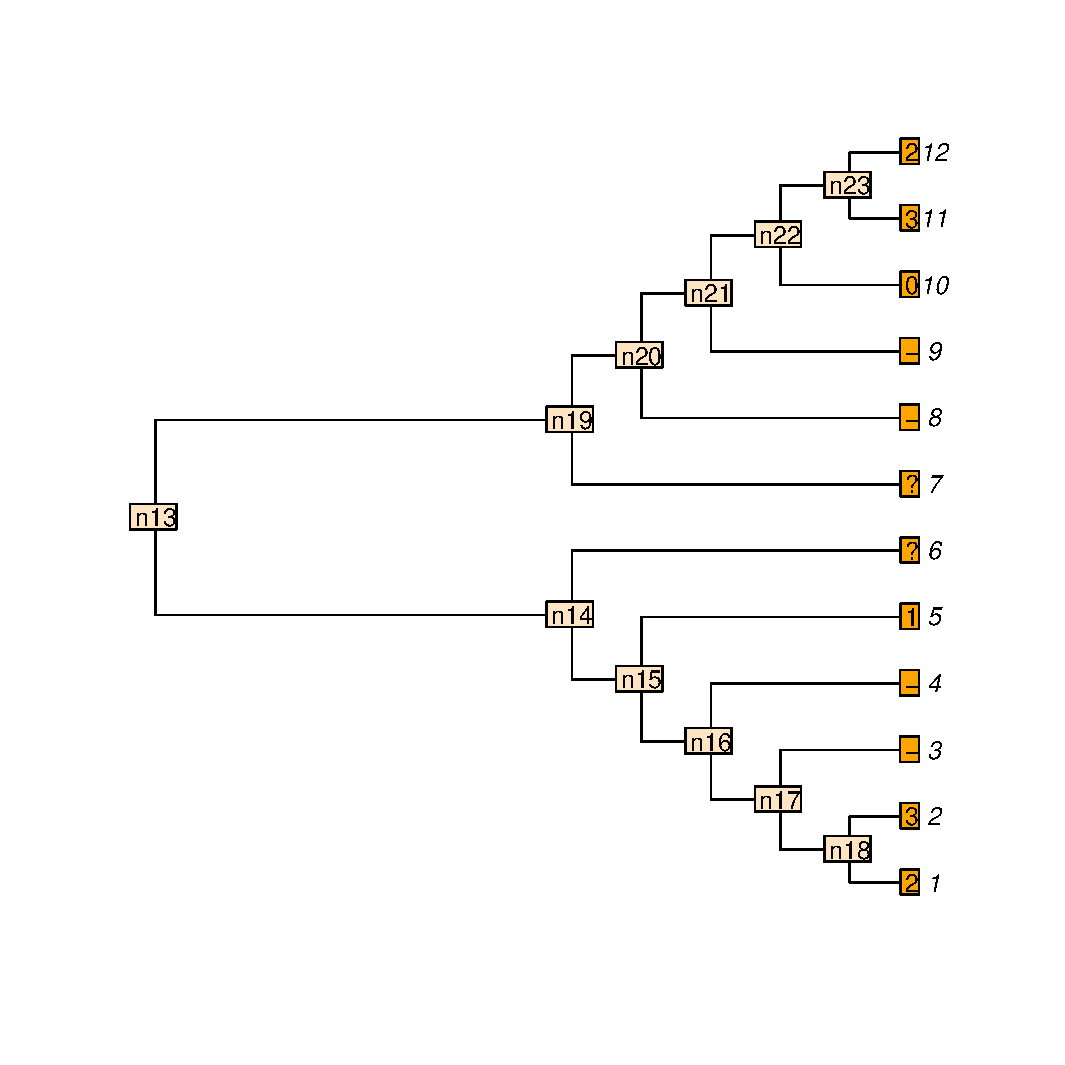
\includegraphics{Inapplicable_data_files/figure-latex/unnamed-chunk-32-1.pdf}

We can use the \texttt{Inapp} package to apply our four-pass
inapplicable algorithm to this character on this tree.

\begin{Shaded}
\begin{Highlighting}[]
\NormalTok{## Loading the Inapp package}
\KeywordTok{library}\NormalTok{(Inapp)}

\NormalTok{## The tree}
\NormalTok{tree <-}\StringTok{ }\KeywordTok{read.tree}\NormalTok{(}\DataTypeTok{text =} \StringTok{"((((((1,2),3),4),5),6),(7,(8,(9,(10,(11,12))))));"}\NormalTok{)}

\NormalTok{## The character}
\NormalTok{character <-}\StringTok{ "23--1??--032"}

\NormalTok{## Applying the NA algorithm}
\NormalTok{matrix <-}\StringTok{ }\KeywordTok{apply.reconstruction}\NormalTok{(tree, character, }\DataTypeTok{method =} \StringTok{"NA"}\NormalTok{)}
\end{Highlighting}
\end{Shaded}

Here is what is happening:

\hypertarget{passes-1-2}{%
\subsection{Passes 1 \& 2}\label{passes-1-2}}

The first two passes are a standard Fitch algorithm applied the the
parent character of the studied character (see
\protect\hyperlink{fitch}{Fitch algorithm}) with a special rule for the
inapplicable state (\texttt{-}).

For the first pass (first downpass):

\begin{itemize}
\tightlist
\item
  If state in common between the two descendants is the inapplicable
  state, but that both have also applicable states, set the node's state
  to be the union between the descendants states (rather than their
  state in common).
\item
  If there is no state in common between the descendants and both
  descendants have applicable states, remove the inapplicable state from
  their union (rather than simply setting the nodal state to their
  union).
\end{itemize}

For the second pass (first uppass):

\begin{itemize}
\tightlist
\item
  If the focal node has both applicable and inapplicable states, set it
  to be the inapplicable state only if its ancestor has also only the
  inapplicable state, else remove the inapplicable state.
\item
  If the focal node has only an inapplicable state and it's ancestor has
  not only the inapplicable state, set it to be the union between it's
  descendants states if their are both applicable, else, leave it as the
  inapplicable state.
\end{itemize}

\begin{Shaded}
\begin{Highlighting}[]
\NormalTok{## Plotting the NA two first passes}
\KeywordTok{plot}\NormalTok{(matrix, }\DataTypeTok{passes =} \KeywordTok{c}\NormalTok{(}\DecValTok{1}\NormalTok{,}\DecValTok{2}\NormalTok{), }\DataTypeTok{counts =} \DecValTok{0}\NormalTok{, }
     \DataTypeTok{legend.pos =} \StringTok{'none'}\NormalTok{, }\DataTypeTok{show.labels =} \KeywordTok{c}\NormalTok{(}\DecValTok{1}\NormalTok{, }\DecValTok{2}\NormalTok{))}
\end{Highlighting}
\end{Shaded}

\begin{figure}
\centering
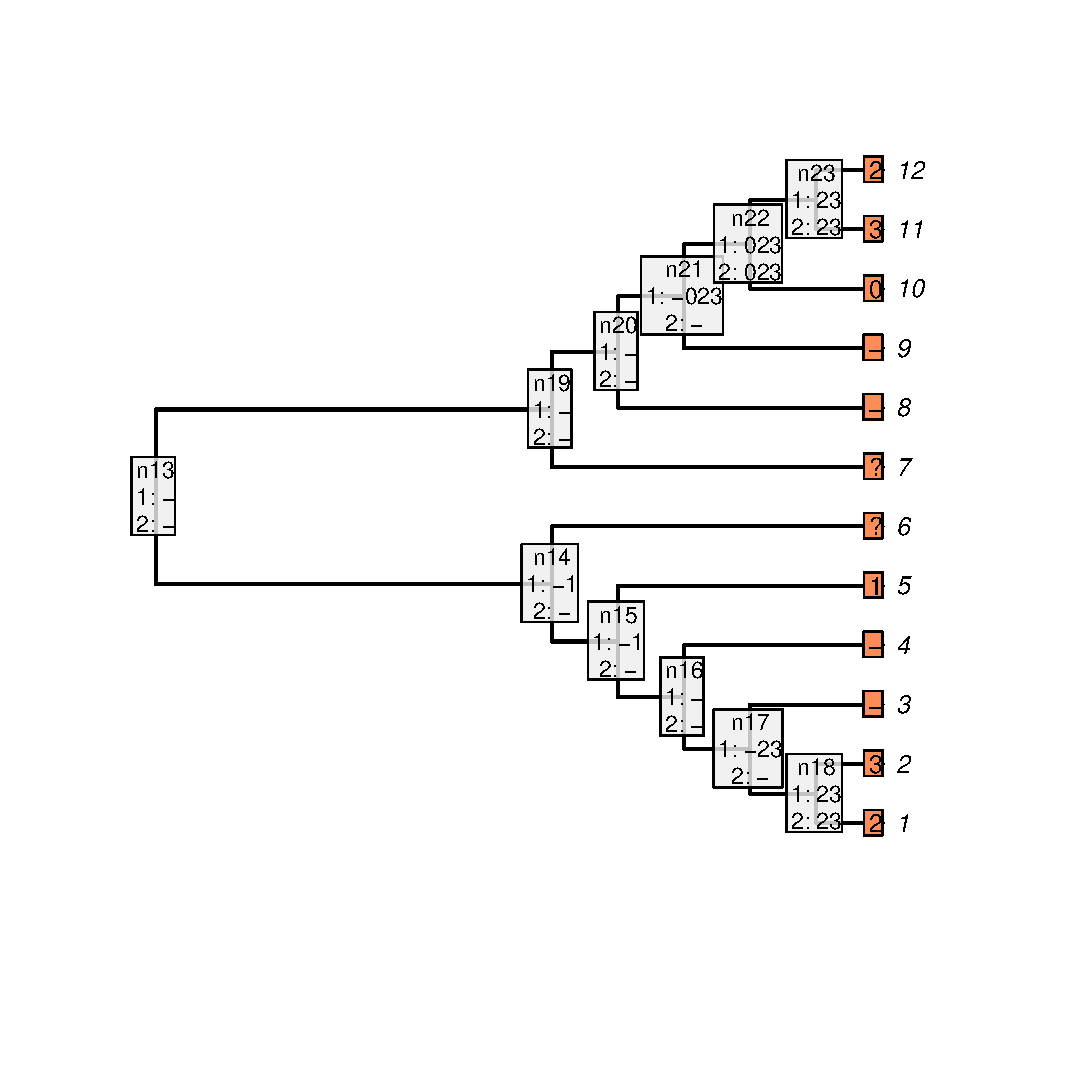
\includegraphics{Inapplicable_data_files/figure-latex/unnamed-chunk-34-1.pdf}
\caption{\label{fig:unnamed-chunk-34}Inapplicable reconstruction after two
passes}
\end{figure}

The parent character can be considered as a binary character ``presence
(\texttt{1}) or absence (\texttt{0}) of a tail'' that would be
\texttt{11001??00111}. The character would be reconstructed as:

\begin{Shaded}
\begin{Highlighting}[]
\NormalTok{## The parent character}
\NormalTok{parent_character <-}\StringTok{ "11001??00111"}

\NormalTok{## Applying the Fitch algorithm}
\NormalTok{matrix_parent <-}\StringTok{ }\KeywordTok{apply.reconstruction}\NormalTok{(tree, parent_character, }\DataTypeTok{method =} \StringTok{"Fitch"}\NormalTok{)}
\KeywordTok{plot}\NormalTok{(matrix_parent, }\DataTypeTok{passes =} \DecValTok{1}\OperatorTok{:}\DecValTok{2}\NormalTok{, }\DataTypeTok{legend.pos=}\StringTok{'none'}\NormalTok{, }\DataTypeTok{show.labels =} \KeywordTok{c}\NormalTok{(}\DecValTok{1}\NormalTok{, }\DecValTok{2}\NormalTok{))}
\end{Highlighting}
\end{Shaded}

\begin{figure}
\centering
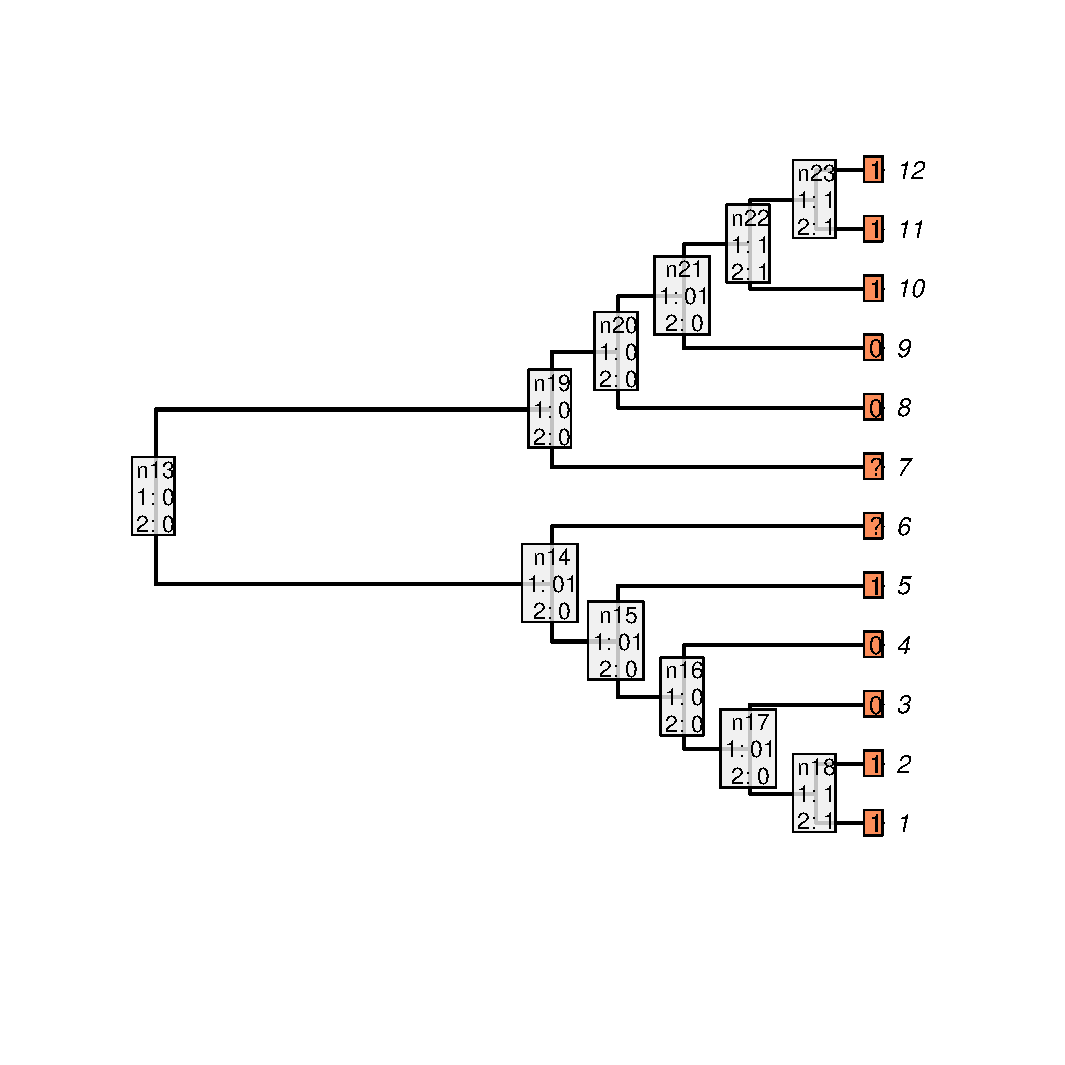
\includegraphics{Inapplicable_data_files/figure-latex/unnamed-chunk-35-1.pdf}
\caption{\label{fig:unnamed-chunk-35}Fitch reconstruction of the parent
character}
\end{figure}

As you can see, both reconstructions are identical: nodes with no tail
are denoted as \texttt{0} in the case of the ``parent character'' and as
\texttt{-} for our current character. Note however that contrary to the
Fitch algorithm, there is no tree score counting in our algorithm for
the two first passes. Indeed, in the case of the Fitch reconstruction of
the ``parent character'', the gain or losses of a tail are counted but
not the changes in states for the subtending character (the tree score
is 3 in Fitch, 5 in our case).

\hypertarget{pass-3}{%
\subsection{Pass 3}\label{pass-3}}

The third pass further resolves ambiguities at nodal states. If the node
is applicable, the standard Fitch downpass comparisons between the
descendants are applied (see \protect\hyperlink{fitch}{Fitch algorithm})
but with the rules relative to the inapplicable state described for the
first downpass above.

During this pass, we can also count the tree score. This score is
composed of both:

\begin{itemize}
\tightlist
\item
  the change in states (e.g.~the change in the colour of the tail)
\item
  the change between applicable and inapplicable regions (e.g.~the
  change in the parent character: a gain or a loss of the tail)
\end{itemize}

The changes of states are calculated the same way as Fitch \textbf{for
the applicable states only}:

\begin{itemize}
\tightlist
\item
  If there is no state in common between both node's descendants and
  that the node, and its descendants have a least one applicable state,
  increment the tree score.
\end{itemize}

\begin{Shaded}
\begin{Highlighting}[]
\KeywordTok{plot}\NormalTok{(matrix, }\DataTypeTok{passes =} \KeywordTok{c}\NormalTok{(}\DecValTok{1}\NormalTok{,}\DecValTok{2}\NormalTok{,}\DecValTok{3}\NormalTok{), }\DataTypeTok{counts =} \DecValTok{2}\NormalTok{, }\DataTypeTok{show.labels =} \KeywordTok{c}\NormalTok{(}\DecValTok{1}\NormalTok{, }\DecValTok{2}\NormalTok{))}
\end{Highlighting}
\end{Shaded}

\begin{figure}
\centering
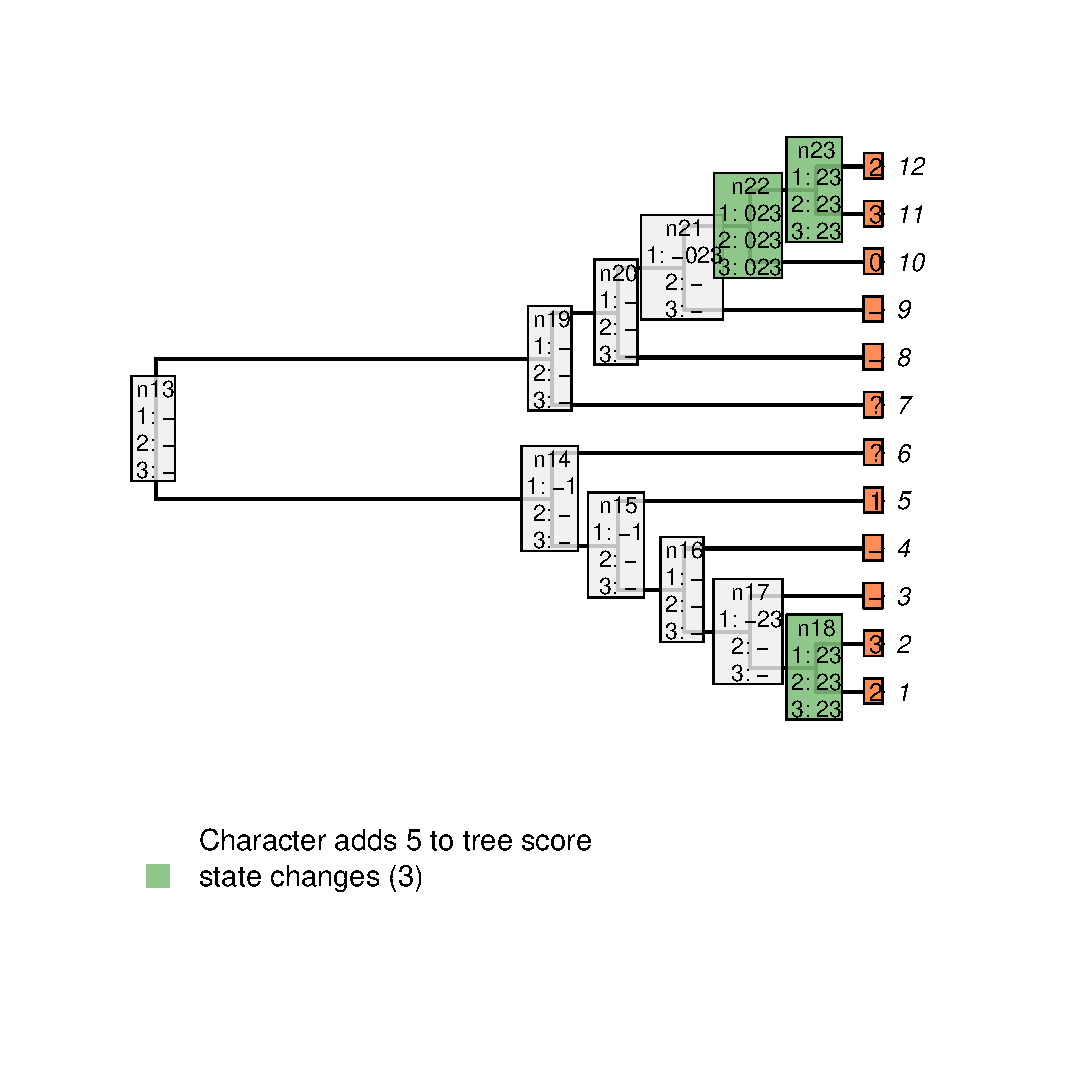
\includegraphics{Inapplicable_data_files/figure-latex/unnamed-chunk-36-1.pdf}
\caption{\label{fig:unnamed-chunk-36}State changes}
\end{figure}

For example, for node \texttt{n23}, there is no state in common between
the tip \texttt{12} (\texttt{2}) and \texttt{11} (\texttt{3}), the tree
score is incremented at this node (case \texttt{1} above). Note,
however, that for node \texttt{n21}, there is no state in common between
node \texttt{n22} (\texttt{023}) and tip \texttt{9} (\texttt{-}) but the
score is not incremented since it does not concern applicable states
only. In other words, there is no change in state at the node
\texttt{n21} from the tail having a colour 0, 2 or 3 to the tail not
being present (\texttt{-}) but rather a change in the parent character
between presence and absence of the tail (present is \texttt{023} and
absent is \texttt{-}).

\hypertarget{tracking-applicable-regions}{%
\subsubsection{Tracking applicable
regions}\label{tracking-applicable-regions}}

To know whether any node leads to a region of applicable states we can
use a ``tracker'' for each node that tells us at any moment whether
descendants of a node contain applicable data or not. When a node is
inapplicable and has a descendant whose lineage leads to applicable
regions, an extra applicable region is implied by the tree. In other
words, following our ``colour of the tail'' character, extra applicable
regions imply independent appearances of the tail somewhere in the
node's descendants.

The tracker is initialised during the \emph{second pass} (first uppass)
and is updated during the \emph{third pass} (second downpass). The
tracker works as follows for each node's left and right descendants:

\begin{itemize}
\tightlist
\item
  If the descendant state is applicable or leads to an applicable
  region, then the node leads to an applicable region; else, it does
  not.
\end{itemize}

The trackers are initialised for each node during the first uppass and
then propagated back down the tree during the second downpass.

Using these trackers, we can then increment the tree score for all
changes that imply a new applicable region. The switch to or from an
inapplicable and applicable region are counted as follows:

\begin{itemize}
\tightlist
\item
  If the node is inapplicable and both descendants lead to regions of
  applicable states, increment the region count.
\item
  If the node is applicable, but has an inapplicable descendant that
  leads to a region of applicable states, increment the region count.
\end{itemize}

\begin{Shaded}
\begin{Highlighting}[]
\KeywordTok{plot}\NormalTok{(matrix, }\DataTypeTok{passes =} \KeywordTok{c}\NormalTok{(}\DecValTok{1}\NormalTok{,}\DecValTok{2}\NormalTok{,}\DecValTok{3}\NormalTok{), }\DataTypeTok{counts =} \DecValTok{1}\NormalTok{, }\DataTypeTok{show.labels =} \KeywordTok{c}\NormalTok{(}\DecValTok{1}\NormalTok{, }\DecValTok{2}\NormalTok{))}
\end{Highlighting}
\end{Shaded}

\begin{figure}
\centering
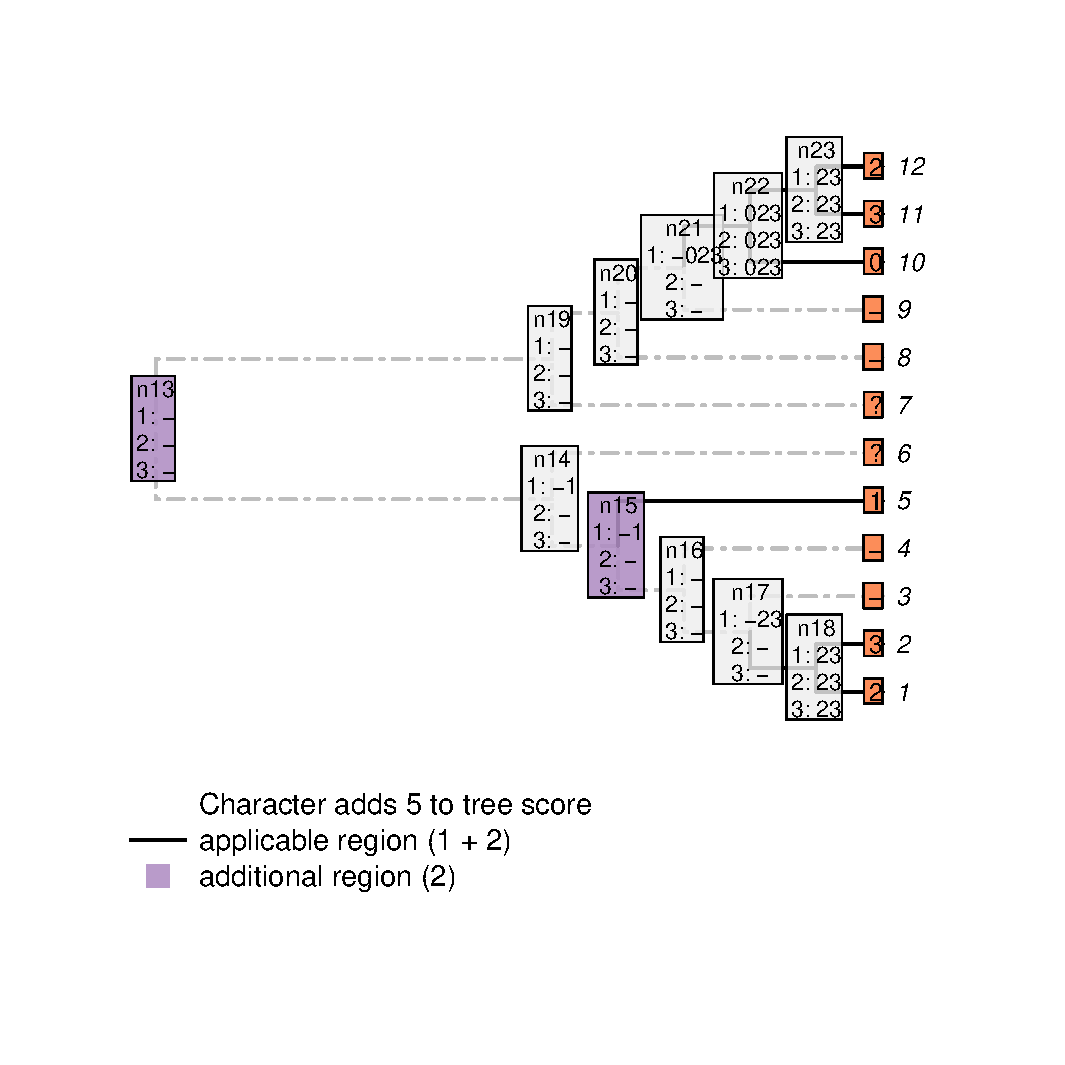
\includegraphics{Inapplicable_data_files/figure-latex/unnamed-chunk-37-1.pdf}
\caption{\label{fig:unnamed-chunk-37}Counting applicable regions}
\end{figure}

For example, node \texttt{n15} is solved as inapplicable but both his
descendants lead to two independent applicable regions (tip \texttt{5}
with the state \texttt{1} and node \texttt{n18} with the states
\texttt{1} and \texttt{2}). This implies an independent change in the
parent character (in our example, tail is absent at node \texttt{n15}
but evolves independently at tip \texttt{5} and node \texttt{n18}).
Conversely, node \texttt{n21} is solved as inapplicable but not both his
descendants lead to independent applicable regions. This node does thus
not imply an independent change in the parent character.

\begin{quote}
Note that the number of applicable regions for a character is always at
least 1 (unless every taxa has the inapplicable state) and therefore, we
only count the \emph{additional} regions.
\end{quote}

Combining both scores -- the number of changes in character states and
the number of additional applicable regions -- we get indeed a total
tree score of 5 for this character on this tree.

\begin{Shaded}
\begin{Highlighting}[]
\NormalTok{## Plotting the NA two first passes}
\KeywordTok{plot}\NormalTok{(matrix, }\DataTypeTok{passes =} \KeywordTok{c}\NormalTok{(}\DecValTok{1}\NormalTok{,}\DecValTok{2}\NormalTok{,}\DecValTok{3}\NormalTok{), }\DataTypeTok{counts =} \KeywordTok{c}\NormalTok{(}\DecValTok{1}\NormalTok{,}\DecValTok{2}\NormalTok{), }\DataTypeTok{show.labels =} \KeywordTok{c}\NormalTok{(}\DecValTok{1}\NormalTok{,}\DecValTok{2}\NormalTok{))}
\end{Highlighting}
\end{Shaded}

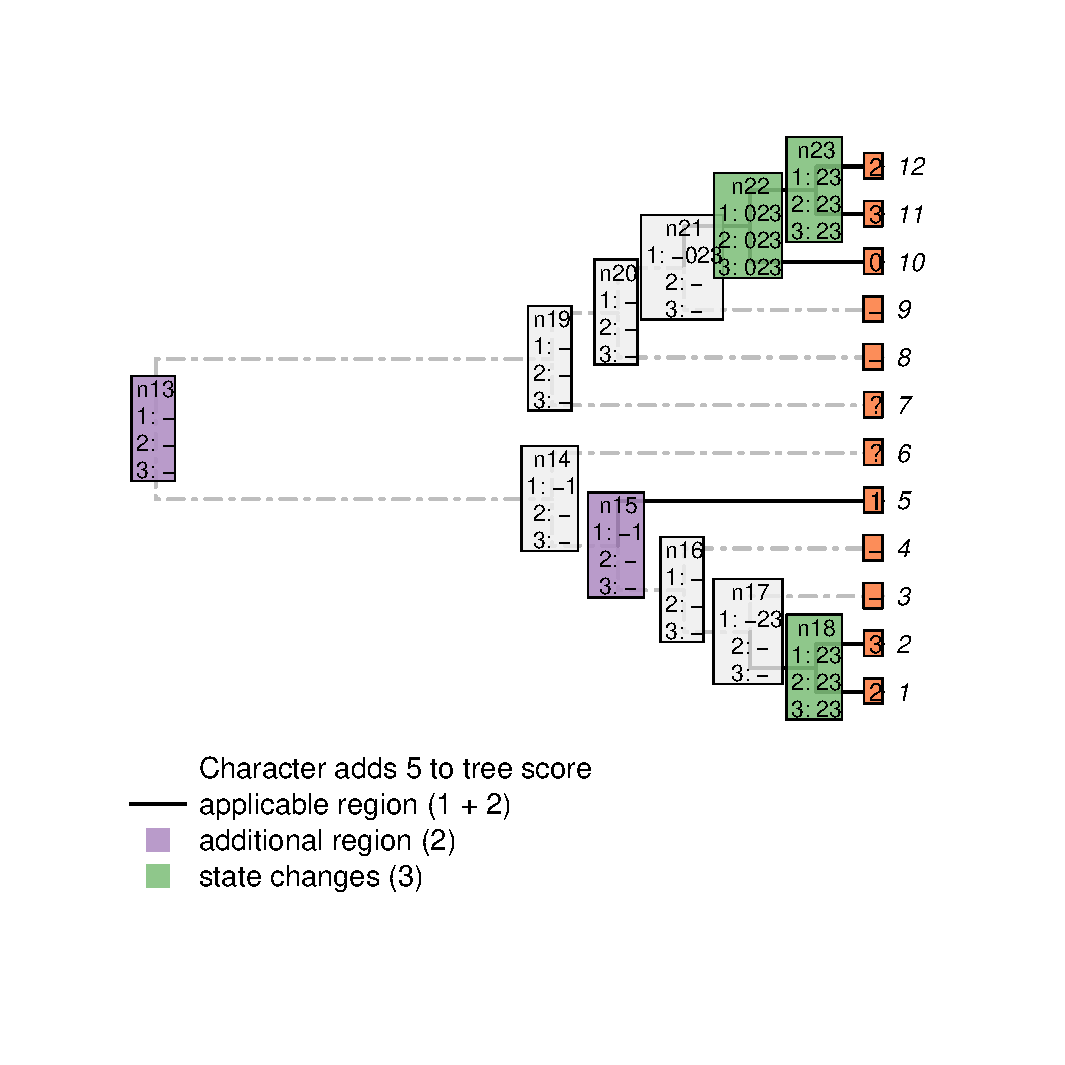
\includegraphics{Inapplicable_data_files/figure-latex/unnamed-chunk-38-1.pdf}

Using the first three passes is enough to get the tree score (while
taking into account inapplicable data!) but does not solve all ancestral
reconstructions. A fourth pass (second uppass) might be necessary to
finalise the node states reconstructions.

\hypertarget{pass-4}{%
\subsection{Pass 4}\label{pass-4}}

In the example above, the node \texttt{n23} is still not correctly
solved after the third pass. It could conceivably be state 0 (with
transformations to states \texttt{2} and \texttt{3} occurring on the
branches leading to tips 11 and 12 respectively). As such, its final
state reconstruction should be \texttt{023}. To reach the correct final
reconstructions, we apply a final pass of the algorithm. This algorithm,
similarly to the second pass of the Fitch algorithm is used to solve
ambiguities in the ancestral nodes reconstructions (although the score
of the tree is already known). It follows these rules and only applies
to nodes and ancestors that have at least one applicable token for
themselves and their ancestor(nodes that are inapplicable are already
solved):

\begin{itemize}
\tightlist
\item
  If there is a state \emph{in common} between the node and its ancestor
  or between the ancestor and the states \emph{in common} of its
  descendants, resolve the node to be this state in common.
\item
  If there is nothing in common between the node and its ancestor or
  between its descendants, solve the node as either:

  \begin{enumerate}
  \def\labelenumi{\arabic{enumi}.}
  \tightlist
  \item
    being the ancestors state if the any of the descendants' have at
    least one inapplicable state but no state in common with the
    ancestor.
  \item
    being the union of the ancestor's and the descendants' states if the
    any of the descendants have at least one inapplicable and have at
    least one state in common with the ancestor.
  \item
    being the union of the ancestor's and the current node states the
    descendants have no inapplicable state.
  \end{enumerate}
\end{itemize}

\begin{Shaded}
\begin{Highlighting}[]
\KeywordTok{plot}\NormalTok{(matrix, }\DataTypeTok{passes =} \KeywordTok{c}\NormalTok{(}\DecValTok{1}\NormalTok{,}\DecValTok{2}\NormalTok{,}\DecValTok{3}\NormalTok{,}\DecValTok{4}\NormalTok{), }\DataTypeTok{counts =} \KeywordTok{c}\NormalTok{(}\DecValTok{1}\NormalTok{,}\DecValTok{2}\NormalTok{), }\DataTypeTok{show.labels =} \KeywordTok{c}\NormalTok{(}\DecValTok{1}\NormalTok{,}\DecValTok{2}\NormalTok{))}\CommentTok{#, col.states=TRUE)}
\end{Highlighting}
\end{Shaded}

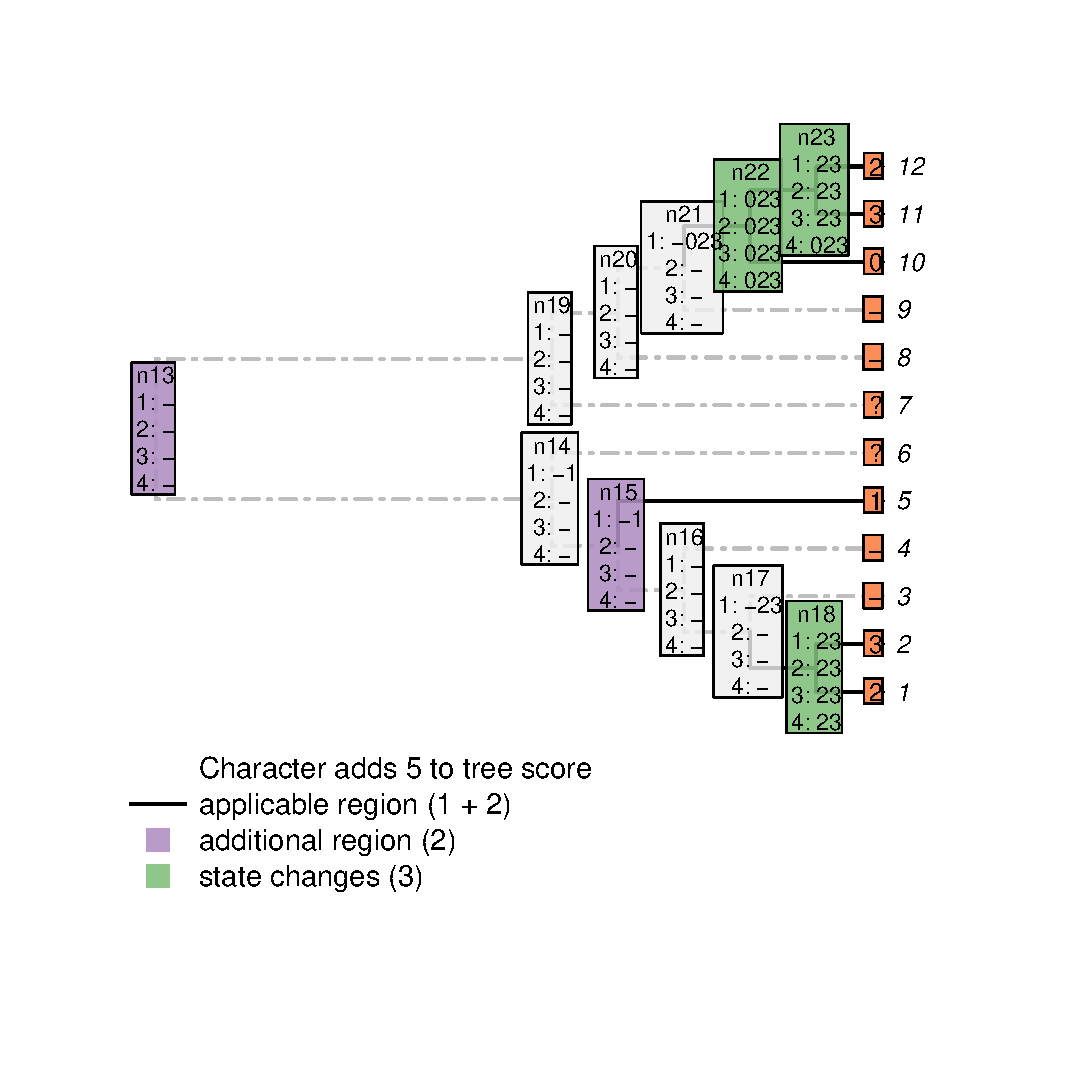
\includegraphics{Inapplicable_data_files/figure-latex/unnamed-chunk-39-1.pdf}

\hypertarget{software}{%
\section{Software implementation}\label{software}}

This algorithm has been implemented in two \texttt{R} packages.
\href{https://github.com/TGuillerme/Inapp}{Inapp} provides an
interactive visualization of how the score of a user-specified tree is
calculated for any character under different approaches to inapplicable
data. This package was used to generate many of the figures in this
document.

\href{https://github.com/ms609/TreeSearch}{TreeSearch} allows for
parsimony tree searches with the inapplicable algorithm
\citep{Brazeau2018}.\\
It includes heuristic search options that make it possible to search
reasonable-sized matrices, and includes an option for equal or implied
weighting.

TreeSearch is a front-end to the
\href{https://github.com/mbrazeau/morphylib}{morphylib} \texttt{C}
library, which will eventually implemented in the standalone
\href{http://www.morphyproject.org/}{Morphy} program for rapid
phylogenetic searches.

\hypertarget{coding}{%
\chapter{Coding data}\label{coding}}

The availability of our algorithm has some implications for how
investigators might choose to code characters.

\hypertarget{multiple-dependencies}{%
\section{Multiple dependencies}\label{multiple-dependencies}}

It's not a problem to have characters dependent on characters that are
dependent on characters. Consider the following characters, whose
descriptions are written in order to emphasize their heirarchical nature
\citep[following the recommendations of][]{Sereno2007}:

\begin{quote}
\begin{enumerate}
\def\labelenumi{\arabic{enumi}.}
\item
  Appendages: (0), absent; (1), present.
\item
  Appendages, termination: (0), blunt; (1), sucker; (2), claw.
\item
  Appendages, suckers, morphology: (0), round; (1), polygonal.
\item
  Appendages, claws, morphology: (0), smooth; (1), serrated.
\end{enumerate}
\end{quote}

The included taxa may or may not bear appendages; if they do, then the
appendages may end either with either claws or suckers, or neither (but
not both). Claws come in two flavours, smooth and serrated; suckers come
in two shapes, rounded and polygonal.

\begin{itemize}
\item
  If character 1 (appendages) is absent, then characters 2--4 are
  inapplicable. Otherwise, charcter 2 (appendage termination) must take
  one of the three applicable values.
\item
  If character 2 (termination) has state 0 (blunt), then characters 3
  and 4 (morphology of sucker / claw) are inapplicable.
\item
  If character 2 (termination) has state 1 (sucker), then character 3
  (sucker morphology) is applicable and character 4 (claw morphology) is
  inapplicable.
\item
  If character 2 (termination) has state 2 (claw), then character 3
  (sucker morphology) is inapplicable and character 4 (claw morphology)
  is applicable.
\end{itemize}

A sample character matrix might look like this:

\begin{table}

\caption{\label{tab:unnamed-chunk-41}Heirarchichal characters}
\centering
\begin{tabular}[t]{l|l|l|l|l|l|l|l|l|l|l|l|l|l}
\hline
  & A & B & C & D & E & F & G & H & I & J & K & L & M\\
\hline
Appendages: (0), absent; (1), present. & 0 & 0 & 0 & 1 & 1 & 1 & 1 & 1 & 1 & 1 & 1 & 1 & 1\\
\hline
Appendage termination: (1), blunt; (2), sucker; (3), claw. & - & - & - & 1 & 1 & 2 & 2 & 2 & 2 & 3 & 3 & 3 & 3\\
\hline
Sucker morphology: (1), smooth; (2), serrated. & - & - & - & - & - & 1 & 1 & 2 & 2 & - & - & - & -\\
\hline
Claw morphology: (1), round; (2), polygonal. & - & - & - & - & - & - & - & - & - & 1 & 1 & 2 & 2\\
\hline
\end{tabular}
\end{table}

Which would plot on a tree thus:

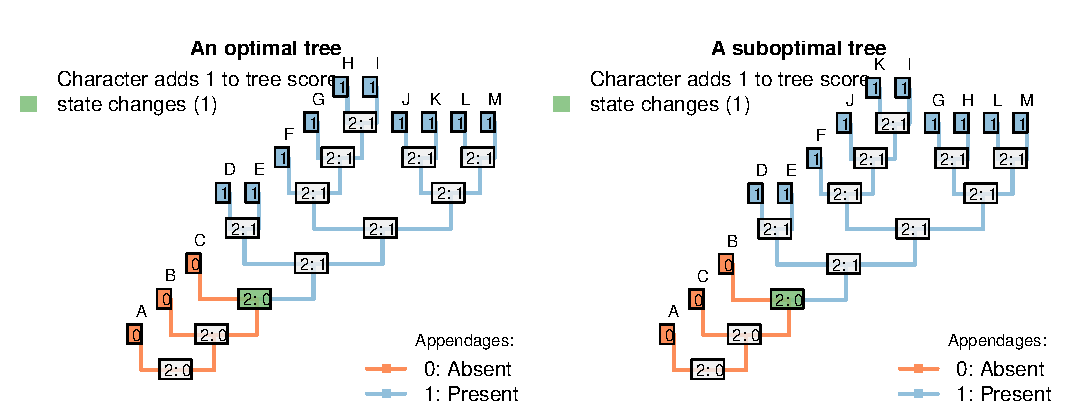
\includegraphics{Inapplicable_data_files/figure-latex/unnamed-chunk-42-1.pdf}
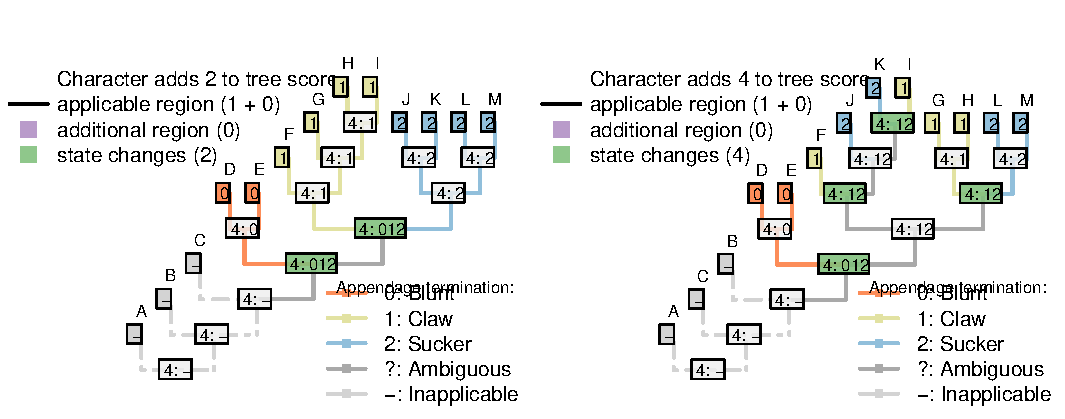
\includegraphics{Inapplicable_data_files/figure-latex/unnamed-chunk-42-2.pdf}
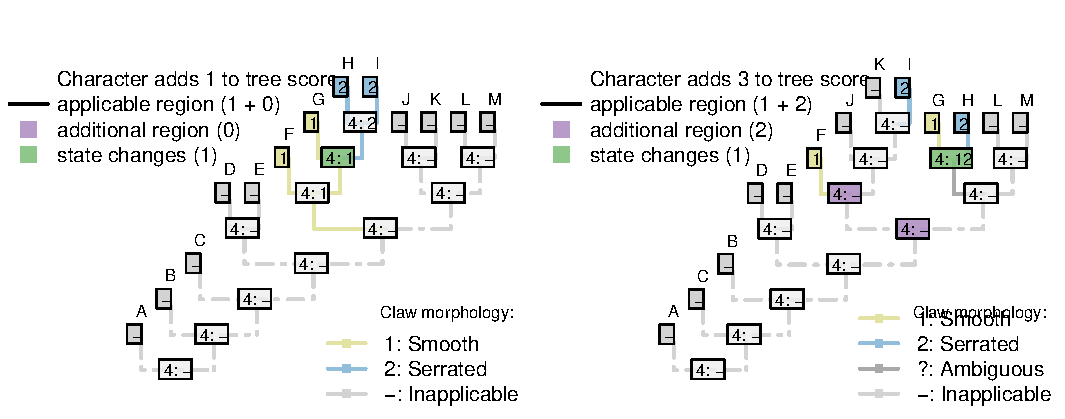
\includegraphics{Inapplicable_data_files/figure-latex/unnamed-chunk-42-3.pdf}
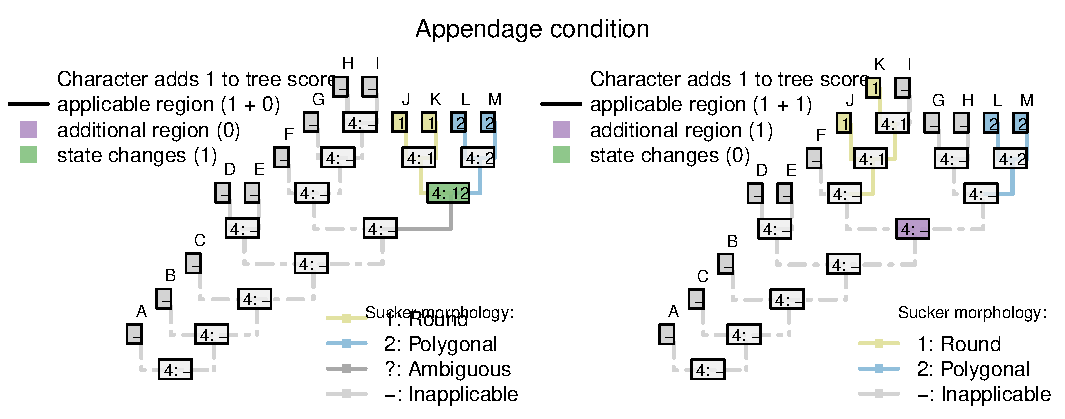
\includegraphics{Inapplicable_data_files/figure-latex/unnamed-chunk-42-4.pdf}

There's no limit to the depth of recursion: one could add a further
character

\begin{quote}
\begin{enumerate}
\def\labelenumi{\arabic{enumi}.}
\setcounter{enumi}{4}
\tightlist
\item
  Appendages, claws, serrations, spacing: (1), regular; (2), irregular.
\end{enumerate}
\end{quote}

that would be inapplicable in all taxa that lacked serrated claws.

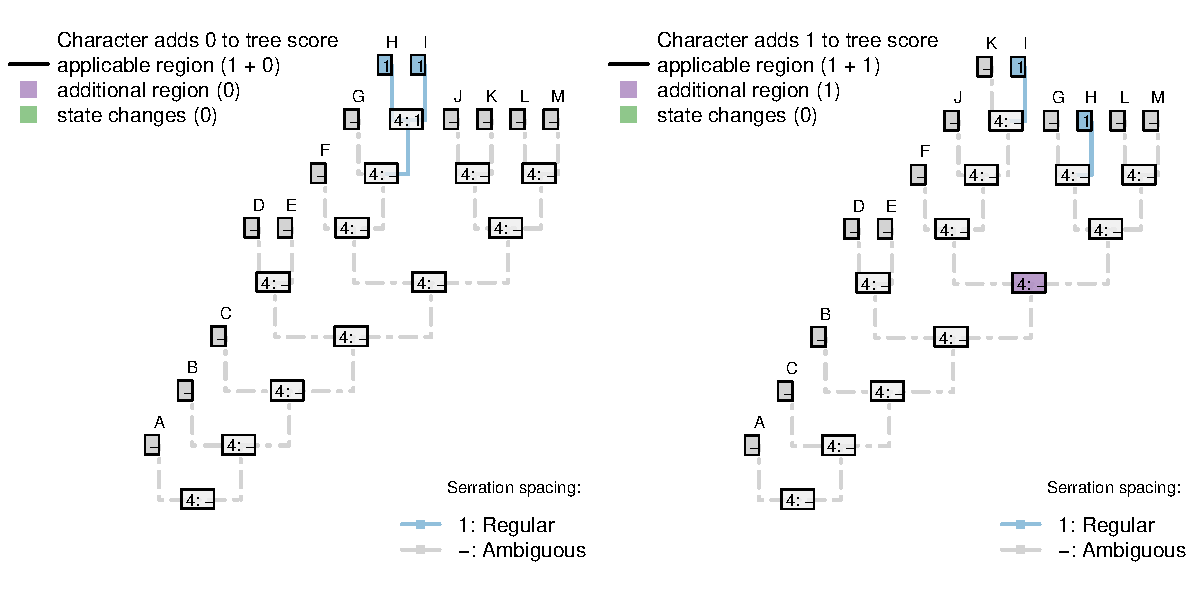
\includegraphics{Inapplicable_data_files/figure-latex/unnamed-chunk-43-1.pdf}

To readers familiar with standard Fitch parsimony, it will be surprising
to notice that the two trees receive a different score for this
invariant character. When our algorithm is employed, invariant
characters that contain inapplicable tokens can inform parsimony.

\hypertarget{invariant-characters-can-inform-parsimony}{%
\section{Invariant characters can inform
parsimony}\label{invariant-characters-can-inform-parsimony}}

Consider a situation in which every tail in the observed taxa is blue --
but the same complex molecular machinery is responsible for this blue
colouration in every taxon.

If its underlying mechanism is considered biologically and
evolutionarily meaningful, then a systematist might opt to include tail
colour as an additional character, even though it is invariant in the
taxa of interest. Reconstructions that attribute this common colouration
to common ancestry will be more parsimonious than those that do not.

\begin{table}

\caption{\label{tab:unnamed-chunk-44}An invariant character, tail colour, contributes as much to tree score as a variable one, body colour.}
\centering
\begin{tabular}[t]{l|l|l|l|l|l|l|l|l}
\hline
  & A & B & C & D & E & F & G & H\\
\hline
Tail: (0), absent; (1), present & 0 & 0 & 0 & 0 & 1 & 1 & 1 & 1\\
\hline
Tail colour: (1), blue; (-), inapplicable & - & - & - & - & 1 & 1 & 1 & 1\\
\hline
Body colour: (1), black; (2), white & 1 & 1 & 2 & 2 & 2 & 2 & 1 & 1\\
\hline
\end{tabular}
\end{table}

Let's compare two trees. The first groups taxa based on the presence of
tails; the other groups taxa based on body colour.

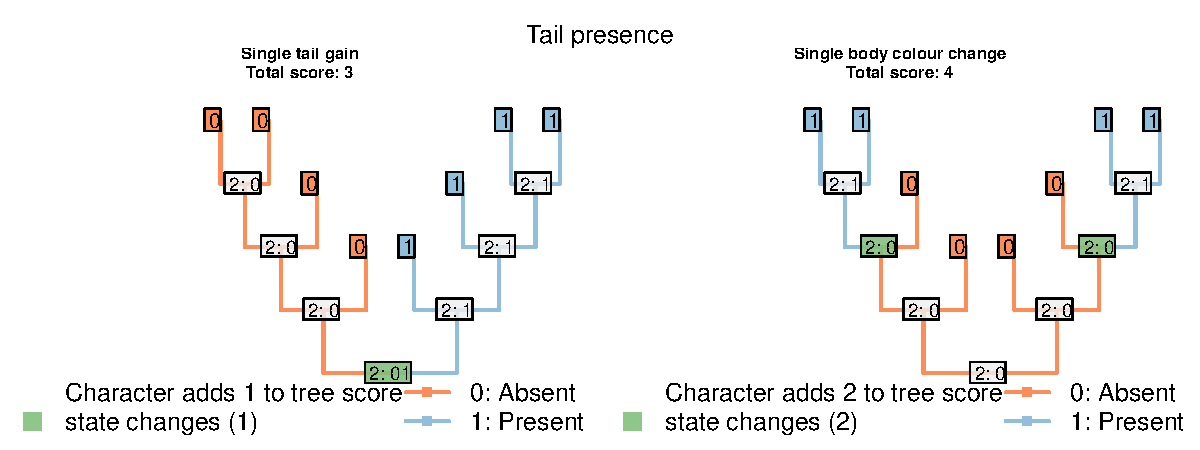
\includegraphics{Inapplicable_data_files/figure-latex/unnamed-chunk-45-1.pdf}
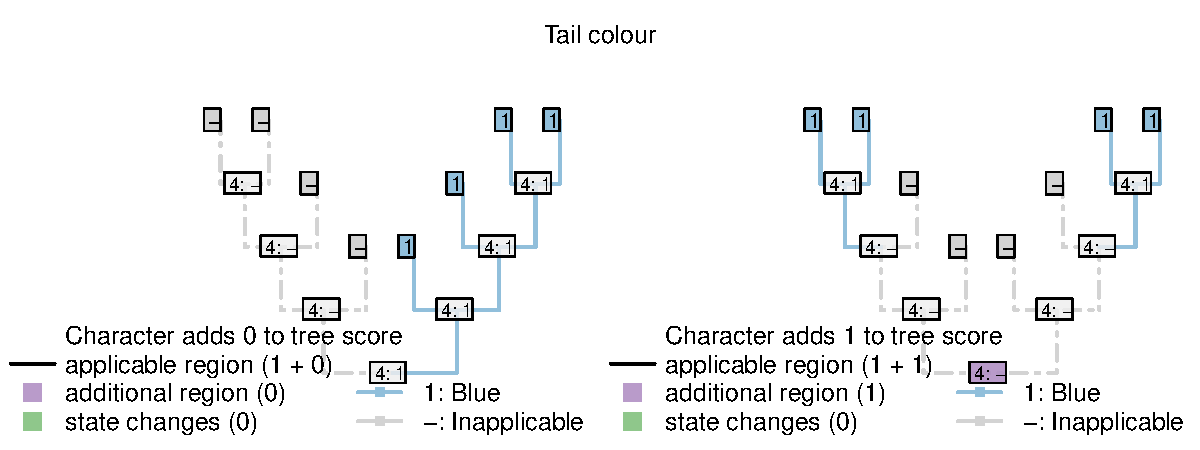
\includegraphics{Inapplicable_data_files/figure-latex/unnamed-chunk-45-2.pdf}
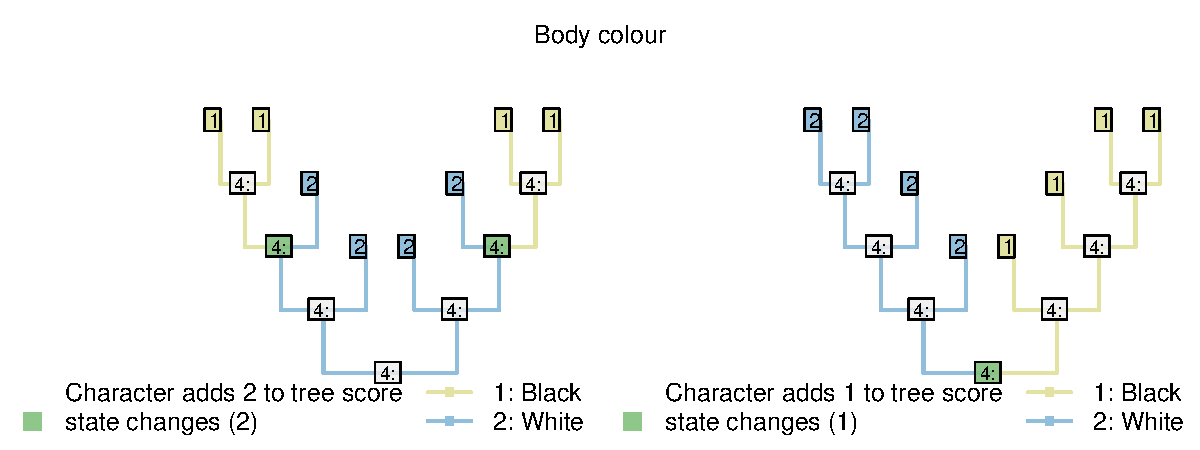
\includegraphics{Inapplicable_data_files/figure-latex/unnamed-chunk-45-3.pdf}

Where the tail has a single origin (one step), blue colouration also
evolves once (zero steps), but body colour must change twice (two steps;
total score = three). But where body colour changes only once (one
step), the tail necessarily arises twice (two steps), meaning two
independent origins of its distinctive blue colouration (one extra
homoplasy; total score = four)

If the invariant tail colour character had not been included, both trees
would have the same score, and there would be nothing to choose between
them. As such, the inclusion or exclusion of invariant characters must
be carefully evaluated: if there is a case that an invariant
(ontologically dependent) character implies an exclusive common ancestry
between those taxa that share it, then it should be included; if not,
then it should be excluded.

\hypertarget{puip}{%
\section{Variable but `parsimony uninformative' characters can inform
parsimony}\label{puip}}

The same effect of course follows if a character has an additional state
that is only observed in one taxon.

\begin{table}

\caption{\label{tab:unnamed-chunk-46}Tail colour is variable but 'parsimony uninformative'}
\centering
\begin{tabular}[t]{l|l|l|l|l|l|l|l|l|l}
\hline
  & A & B & C & D & E & F & G & H & I\\
\hline
Tail: (0), absent; (1), present & 0 & 0 & 0 & 0 & 1 & 1 & 1 & 1 & 1\\
\hline
Tail colour: (1), red; (2), blue; (-), inapplicable & - & - & - & - & 1 & 1 & 1 & 1 & **2**\\
\hline
Body colour: (1), black; (2), white & 1 & 1 & 2 & 2 & 2 & 2 & 1 & 1 & 1\\
\hline
\end{tabular}
\end{table}

Any tree that implies that blueness evolves multiple times will incur an
additional penalty that would not have been encountered had the tail
colour character been omitted.

\begin{figure}
\centering
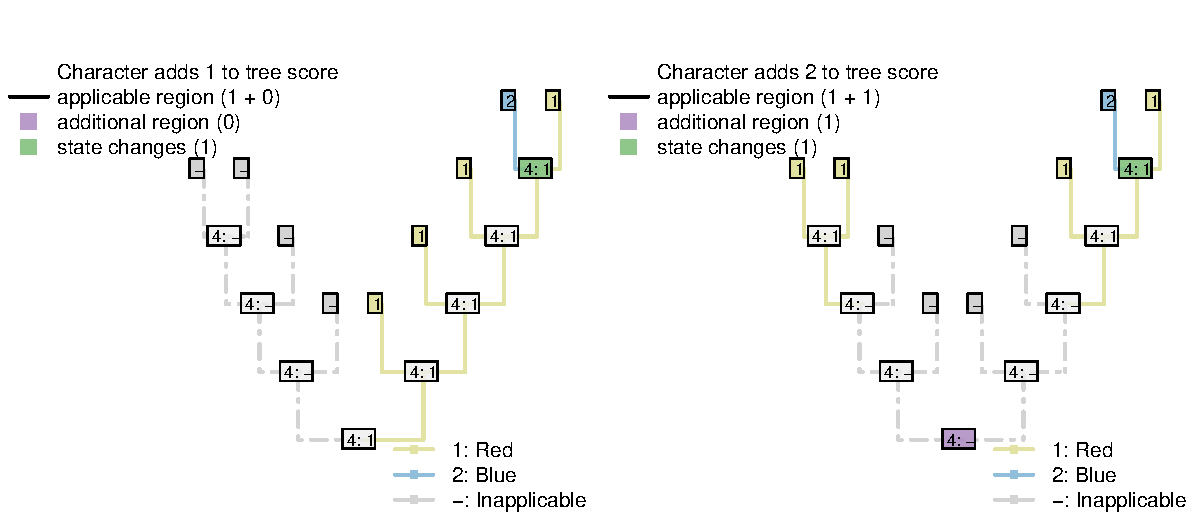
\includegraphics{Inapplicable_data_files/figure-latex/unnamed-chunk-47-1.pdf}
\caption{\label{fig:unnamed-chunk-47}Tail colour}
\end{figure}

\hypertarget{this-may-not-be-desirable-in-neomorphic-characters}{%
\section{This may not be desirable in neomorphic
characters}\label{this-may-not-be-desirable-in-neomorphic-characters}}

The more general rule is that any tree that reconstructs the same state
arising twice, independently, in an ontologically dependent character
will incur a penalty relative to one that reconstructs that same state
arising once.

With transformational characters, this is often a desideratum -- as
discussed above.

In certain neomorphic characters, however, it may not be desirable to
penalise trees in which the \emph{absence} of a character arises
multiple times.

Let us imagine that there is a biological reason to believe that tails
in a particular group lacked poisoned barbs when they first evolved:
that is, poisoned barbs are an evolutionary innovation that can only be
added to a tail once a tail is already present.

\begin{table}

\caption{\label{tab:unnamed-chunk-48}A neomorphic character, poison barbs, present in some but not all tails}
\centering
\begin{tabular}[t]{l|l|l|l|l|l|l|l|l|l}
\hline
  & A & B & C & D & E & F & G & H & I\\
\hline
Tail: (0), absent; (1), present & 0 & 0 & 0 & 1 & 1 & 1 & 1 & 1 & 1\\
\hline
Tail, poison barbs: (-), inapplicable; (0), absent; (1), present & - & - & - & 0 & 0 & 0 & 0 & 1 & 1\\
\hline
\end{tabular}
\end{table}

\hypertarget{three-scenarios}{%
\subsection{Three scenarios}\label{three-scenarios}}

The presence of poison barbs obviously contains grouping information --
a reconstruction that attribute the presence of posion barbs to a single
evolutionary gain in a common ancestor is parsimonious with respect to
that character (even if it is less parsimonious with respect to another
-- e.g.~the presence or absence of a tail).

\begin{figure}
\centering
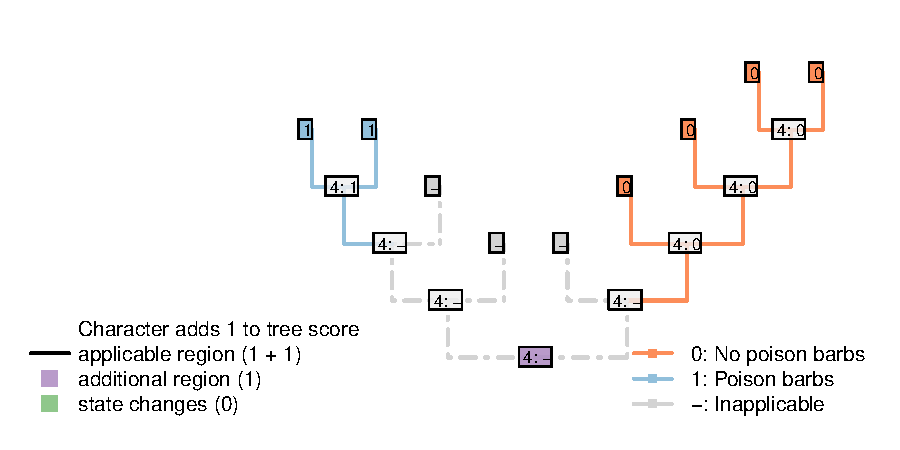
\includegraphics{Inapplicable_data_files/figure-latex/unnamed-chunk-50-1.pdf}
\caption{\label{fig:unnamed-chunk-50}One tail with barbs, one without}
\end{figure}

Consider a reconstruction in which a tail evolved twice, and barbs
evolved twice. Here, the duplicate origin of barbs (as well as the
duplicate origin of the tail) makes this reconstruction less
parsimonious.

\begin{figure}
\centering
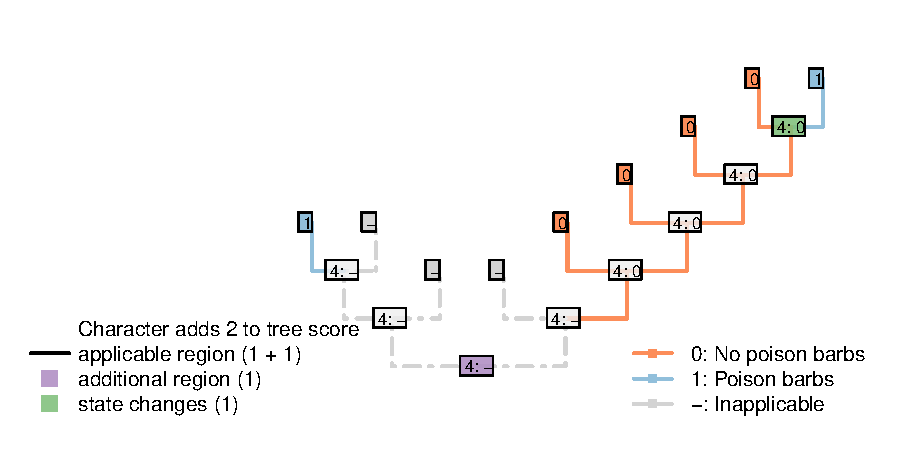
\includegraphics{Inapplicable_data_files/figure-latex/unnamed-chunk-51-1.pdf}
\caption{\label{fig:unnamed-chunk-51}Two barb appearances}
\end{figure}

But what about a situation in which a tail evolved twice, and lacked
barbs each time it evolved? Coding this character as transformational
penalises the duplicate origin of the state ``no poison barbs'', making
this reconstruction less parsimonious.

If we expect a tail, when it evolves, to lack barbs, then the second
origin of ``no barbs'' does not represent a homoplasy: it's not a
feature that has evolved twice, but rather an observation that something
has \emph{not} evolved twice.

The absence of poison barbs in the two ancestral tail-bearers has been
inherited from a common ancestor that did not itself bear tail barbs (by
virtue, in this instance, of not bearing a tail). This second
non-origination should not, therefore, be penalized in this situation.

\begin{figure}
\centering
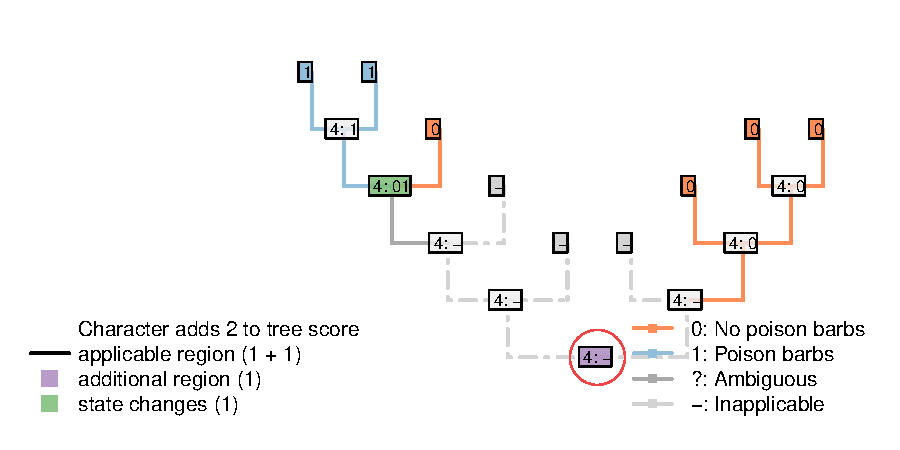
\includegraphics{Inapplicable_data_files/figure-latex/unnamed-chunk-52-1.pdf}
\caption{\label{fig:unnamed-chunk-52}Two barbless appearances: second
absence is penalized}
\end{figure}

This problem has arisen because the inapplicable token has been used in
a character that is, in fact, applicable.

The statement ``A tail is absent; the tail is red'' is not logically
consistent, which is why the inapplicable token is necessary. In
contrast, the statement ``A tail is absent; tail barbs are absent''
\emph{is} logically consistent, and the inapplicable token is not
necessary. Instead, the `absence' token should be employed instead of
the inapplicable:

\begin{figure}
\centering
\includegraphics{Inapplicable_data_files/figure-latex/unnamed-chunk-53-1.pdf}
\caption{\label{fig:unnamed-chunk-53}Two barbless appearances}
\end{figure}

The point here is that the inapplicable token ought only to be used in
tips where a character description literally does not apply. As an
example, De Laet \citeyearpar{DeLaet2017} contends that the character
``Tail: absent/present'' is inapplicable in an angiosperm. We disagree.
Angiosperms do not have tails. ``Tail'' should be coded as absent in
angiosperms.

One way to emphasize this distinction in character matrices is to
reserve the \texttt{0} token to denote absence, and denoting states of
transformational characters using the positive integers:

\begin{table}

\caption{\label{tab:unnamed-chunk-54}Recommended coding: state 0 reserved for absence; states 1 and 2 used for (transformational) tail colour character.}
\centering
\begin{tabular}[t]{l|l|l|l|l|l|l|l|l|l}
\hline
  & A & B & C & D & E & F & G & H & I\\
\hline
Tail: (0), absent; (1), present & 0 & 0 & 0 & 1 & 1 & 1 & 1 & 1 & 1\\
\hline
Tail, poison barbs: (0), absent; (1), present & 0 & 0 & 0 & 0 & 0 & 0 & 0 & 1 & 1\\
\hline
Tail, colour: (-), inapplicable; (1), red; (2), blue & - & - & - & 1 & 1 & 1 & 2 & 2 & 2\\
\hline
\end{tabular}
\end{table}

One implication of this coding strategy is that the loss of a tail (a
single evolutionary event) causes the loss of all contingent characters
-- characters are not independent.

\begin{figure}
\centering
\includegraphics{Inapplicable_data_files/figure-latex/unnamed-chunk-55-1.pdf}
\caption{\label{fig:unnamed-chunk-55}Presence of a tail and presence of
poison barbs will have the same distribution if all tails have poison
barbs. Loss and subsequent re-gain of a tail implies the same loss and
re-gain of barbs.}
\end{figure}

If a poisoned tail was present in a lineage, then lost, then re-gained,
would one expect the re-gained tail to also re-gain its poisoned barbs?
One could spend some time evaluating whether this behaviour has a
biological underpinning, or whether it is desirable -- is a
reconstruction that invokes the loss of a complex tail more parsimonious
than one that invokes the loss of a simple tail?

Indeed, it would be straightforwards to construct an algorithm that does
not penalise losses where the loss corresponds to the inferred loss of a
parent character.

The underlying issue, however, is that both parsimony and the Mk model
assume character independence; it is perhaps more fruitful to focus
effort on developing models of evolution that take proper account of
character non-independence.

\hypertarget{does-absence-contain-phylogenetic-information}{%
\subsection{Does absence contain phylogenetic
information?}\label{does-absence-contain-phylogenetic-information}}

In some cases, the absence of a feature (e.g.~serrations) may represent
a transformational character and should thus be coded as such. But this
decision is significant, and merits careful thought. A researcher may or
may not be justified in including properties of a tail that occur in
only one, or even in none, of the taxa of interest, for if absence is
informative for parsimony, then such characters will influence tree
topology: \protect\hyperlink{puip}{parsimony uninformative characters
inform parsimony}.

\begin{table}

\caption{\label{tab:unnamed-chunk-56}Absences treated as transformational characters}
\centering
\begin{tabular}[t]{l|l|l|l|l|l|l|l}
\hline
  & A & B & C & D & E & F & G\\
\hline
Tail: (0), absent; (1), present & 0 & 0 & 0 & 1 & 1 & 1 & 1\\
\hline
Tail, margin: (-), inapplicable; (1), smooth; (2), serrated & - & - & - & \{12\} & \{12\} & 1 & 1\\
\hline
Tail, glow-in-the-dark pigment: (-), inapplicable; (1), absent; (2), present & - & - & - & \{12\} & \{12\} & 1 & 1\\
\hline
Tail, ability to generate electricity: (-), inapplicable; (1), absent; (2), present & - & - & - & \{12\} & \{12\} & 1 & 1\\
\hline
\end{tabular}
\end{table}

Note that each of the unobserved (i.e.~always-absent) characters
provides evidence against independent origins of the tail, in favour of
independent losses:

\includegraphics{Inapplicable_data_files/figure-latex/unnamed-chunk-57-1.pdf}

Under the simple matrix presented above, the left-hand tree receives a
score of five (two independent gains of the tail, plus the three
ontologically dependent characters with an additional step each),
whereas the right-hand tree scores but three (three independent losses
of the tail; no steps in the ontologically dependent characters), making
it more parsimonious.

If the three ontologically-dependent characters were coded as `absent'
(instead of inapplicable) when the tail was absent, then the left-hand
tree would be preferred (with a score of 2 vs.~3).

The two trees are equally parsimonious (both scoring three) if tail
margin is treated as a trasnformational character (inapplicable when
tail absent) and the other characters are treated as neomorphic (absent
when tail absent).

\begin{table}

\caption{\label{tab:unnamed-chunk-58}Recommended coding: Absences treated as neomorphic characters were appropriate}
\centering
\begin{tabular}[t]{l|l|l|l|l|l|l|l}
\hline
  & A & B & C & D & E & F & G\\
\hline
Tail: (0), absent; (1), present & 0 & 0 & 0 & 1 & 1 & 1 & 1\\
\hline
Tail, margin: (1), smooth; (2), serrated & - & - & - & \{12\} & \{12\} & 1 & 1\\
\hline
Tail, glow-in-the-dark pigment: (-), inapplicable; (0), absent; (1), present & 0 & 0 & 0 & \{01\} & \{01\} & 0 & 0\\
\hline
Tail, ability to generate electricity: (-), inapplicable; (0), absent; (1), present & 0 & 0 & 0 & \{01\} & \{01\} & 0 & 0\\
\hline
\end{tabular}
\end{table}

\hypertarget{ambiguity}{%
\chapter{Coding ambiguity}\label{ambiguity}}

Ambiguous data does not pose a problem for the algorithm, but the nature
of the ambiguity must be considered when scoring a character.

\hypertarget{principal-character-ambiguous}{%
\section{Principal character
ambiguous}\label{principal-character-ambiguous}}

If it's not clear whether or not a taxon has a tail, then tail colour
should be coded as \texttt{?}, denoting that any possible token
(including the inapplicable token) may be the most parsimonious for the
tail.

In trees in which the tail can be reconstructed as present, the
ambiguous tip will be reconstructed as having a tail of the appropriate
colour:

\includegraphics{Inapplicable_data_files/figure-latex/unnamed-chunk-60-1.pdf}

In trees in which the tail cannot be reconstructed as present without
inferring a homoplasious origin, the tail colour will be reconstructed
as inapplicable:

\includegraphics{Inapplicable_data_files/figure-latex/unnamed-chunk-61-1.pdf}

\hypertarget{principal-character-known}{%
\section{Principal character known}\label{principal-character-known}}

If a taxon is known to have a tail, there are two scenarios for
ontologically dependent transformational characters:

\hypertarget{subordinate-character-has-finite-states}{%
\subsection{Subordinate character has finite
states}\label{subordinate-character-has-finite-states}}

If the subordinate character must take one of a finite set of values,
then the unobserved property of the tail is known to belong to these
values and should be coded accordingly.

For example:

\begin{quote}
Tail: (0), absent; (1), present

Tail margin: (0), smooth; (1), serrated.
\end{quote}

Assume that the tail margin must either be smooth or serrated, and there
is no reason to assume that either state is ancestral (i.e.~the
character is strictly transformational). Tail margin should then be
coded as \texttt{\{01\}}: i.e.~the tail is known to have taken one of
the two states 0 or 1.

\hypertarget{subordinate-character-may-have-unobserved-states}{%
\subsection{Subordinate character may have unobserved
states}\label{subordinate-character-may-have-unobserved-states}}

A more complicated situation arises where a subordinate character may
have unobserved states, as with

\begin{quote}
Tail colour: (0), red; (1), blue.
\end{quote}

A taxon that is known to have a tail, but whose tail colour is
uncertain, should generally be coded as \texttt{?}.

Coding it as \texttt{\{01\}} would be appropriate if the tail was known
to certainly be homologous with other tails in the dataset, in which
case it would be most parsimonious to assume that the tail colour is the
same colour as the ancestor of the tip, which was necessarily either red
or blue.

\includegraphics{Inapplicable_data_files/figure-latex/unnamed-chunk-62-1.pdf}

But if, as will more often be the case, homology of the tails is not
known \emph{a priori}, then it is possible that this taxon has a tail
that is not homologous with any other tail whose colour has been
observed.

In this case, coding the tail colour as \texttt{\{01\}} denotes that the
tail is the same colour as a tail that has already been observed. This
means that the independent origin of the tail also represents an
independent origin of this particular colour -- and hence an instance of
homoplasy.

\includegraphics{Inapplicable_data_files/figure-latex/unnamed-chunk-63-1.pdf}

Coding the tail colour as \texttt{?} allows the possibility that the
independently-evolved tail has a different colour to the tails already
observed -- green, perhaps. Reconstructing the tail colour as a colour
that has not already been observed avoids an instance of homoplasy, and
is therefore more parsimonious.

In the case that the unknown tail evolved independently and was green,
the original character formulation -- which only provides tokens for red
and blue tails -- cannot be applied and is thus inapplicable. Our
algorithm will thus reconstruct tail colour as being inapplicable in
such a taxon.

\includegraphics{Inapplicable_data_files/figure-latex/unnamed-chunk-64-1.pdf}

\hypertarget{recommendation}{%
\section{Recommendation}\label{recommendation}}

We therefore recommend the following coding schema for ambiguous tips
where the tail is known to be present, ambiguous, or known to be absent:

\begin{table}

\caption{\label{tab:unnamed-chunk-65}Recommended coding for unknown contingent characters}
\centering
\begin{tabular}[t]{l|l|l|l}
\hline
  & Present & Unknown & Absent\\
\hline
Tail: (0), absent; (1), present. & 1 & ? & 0\\
\hline
Tail margin: (0), smooth; (1), serrated. & \{01\} & ? & -\\
\hline
Tail colour: (0), red; (1), blue. & ? & ? & -\\
\hline
\end{tabular}
\end{table}

``Tail margin'' represents a character that can only take the states
observed (smooth or serrated), whereas tail colour represents a
character that may take an unobserved state (e.g.~green).

\hypertarget{examples}{%
\chapter{Examples}\label{examples}}

This vignette describes how the algorithm approaches some example trees.
We follow the example of a tail coded using two characters:

\begin{quote}
Tail: (0), absent; (1), present;

Tail colour: (0), red; (1), blue.
\end{quote}

\hypertarget{some-caterpillars}{%
\section{Some caterpillars}\label{some-caterpillars}}

First we'll address some pectinate ``caterpillar'' trees, in which eight
taxa have tails (and eight do not), four of which are red, four of which
are blue.

An optimal tree with this character invokes a single origin of the tail,
and a single change in tail colour, thus incurring a score of two. Here
is one example:

\begin{figure}
\centering
\includegraphics{Inapplicable_data_files/figure-latex/unnamed-chunk-68-1.pdf}
\caption{\label{fig:unnamed-chunk-68}An optimal tree: Total score 2}
\end{figure}

If we insist that the tail evolves twice, then the best score is
accomplished by reconstructing a different colour of tail in each of the
two regions in which the tail is present. On a caterpillar tree, this
means the loss of a tail that has one colour, and an independent
innovation in a tail-less taxon of a tail that has a different colour:

\begin{figure}
\centering
\includegraphics{Inapplicable_data_files/figure-latex/unnamed-chunk-69-1.pdf}
\caption{\label{fig:unnamed-chunk-69}Two tail innovations: Total score 2
(best possible)}
\end{figure}

Under the parsimony criterion, it is considered less optimal if a tail,
when it re-evolves, happens to independently re-evolve a colour that has
already been observed -- ``blueness'' has evolved twice on the following
tree, meaning that the second innovation of ``blueness'' represents an
instance of homoplasy.

\begin{figure}
\centering
\includegraphics{Inapplicable_data_files/figure-latex/unnamed-chunk-70-1.pdf}
\caption{\label{fig:unnamed-chunk-70}Tree A: Total score 4}
\end{figure}

\hypertarget{three-equally-suboptimal-alternatives}{%
\section{Three equally suboptimal
alternatives}\label{three-equally-suboptimal-alternatives}}

The following three trees differ in the number of innovations of the
tail that are implied, and the number of changes in tail colour. All are
equally parsimonious.

Under the first, our algorithm reconstructs the tail as ancestrally
present, being lost on edge 2, gained on edge 5, lost in tips H and I,
lost on edge 11, and gained on edge 14 (a total of six homoplasies). It
further reconstructs independent, homoplastic origins of tail redness on
edge 5, tail blueness on edge 14, and a change in tail colour from red
to blue somewhere between edges 7 and 9 (three homoplasies).

\begin{figure}
\centering
\includegraphics{Inapplicable_data_files/figure-latex/unnamed-chunk-71-1.pdf}
\caption{\label{fig:unnamed-chunk-71}Tree B: Total score 9}
\end{figure}

In the second, our algorithm reconstructs the tail as ancestrally
present, being lost in tips B, D, E, H, and I, and on edge 11, before
being independently gained on edge 14 (a total of seven homoplasies).\\
It further reconstructs an independent, homoplastic origins of tail
blueness on edge 14, and a change in tail colour from red to blue
somewhere between edges 7 and 9 (two homoplasies).

\begin{figure}
\centering
\includegraphics{Inapplicable_data_files/figure-latex/unnamed-chunk-72-1.pdf}
\caption{\label{fig:unnamed-chunk-72}Tree C: Total score 9}
\end{figure}

The third configuration reconstructs the tail as ancestrally present,
being lost in tips B, D, F, H, J, L, N and P (a total of eight
homoplastic losses). It further reconstructs a single change in tail
colour from red to blue on edge 8.

\begin{figure}
\centering
\includegraphics{Inapplicable_data_files/figure-latex/unnamed-chunk-73-1.pdf}
\caption{\label{fig:unnamed-chunk-73}Tree D: Total score 9}
\end{figure}

\hypertarget{a-better-caterpillar-tree}{%
\section{A better caterpillar tree}\label{a-better-caterpillar-tree}}

The tree below obtains a better score than any of the previous three: it
implies a loss of the tail at edge 2, a gain at edge 6, a loss at edge
10, and a gain at edge 14; it invokes a homoplastic origin of redness at
edge 6, one of blueness at edge 14, and a change in colour at edge 8,
for a combined score of 7.

\begin{figure}
\centering
\includegraphics{Inapplicable_data_files/figure-latex/unnamed-chunk-74-1.pdf}
\caption{\label{fig:unnamed-chunk-74}Tree E: Total score 7}
\end{figure}

\hypertarget{de-laets-caterpillars}{%
\section{De Laet's caterpillars}\label{de-laets-caterpillars}}

De Laet \citeyearpar{DeLaet2017} identifies a corner case in which our
algorithm \citep{Brazeau2018} will not reconstruct every
equally-parsimonious character reconstruction. Below is a simplified
version of his example:

\begin{table}

\caption{\label{tab:unnamed-chunk-76}Coding}
\centering
\begin{tabular}[t]{l|l|l|l|l|l|l|l|l}
\hline
  & A & B & C & D & E & F & G & H\\
\hline
Tail: (0), absent; (1), present. & 0 & 1 & 1 & ? & 0 & 0 & 1 & 1\\
\hline
Tail, colour: (1), red; (2),blue. & - & 1 & 1 & ? & - & - & 2 & 2\\
\hline
\end{tabular}
\end{table}

When optimising tail colour, we reconstruct the tail as present at all
internal nodes, with independent losses of the tail in each of the three
tailless taxa (i.e.~edges 1, 9, 11).

\includegraphics{Inapplicable_data_files/figure-latex/unnamed-chunk-77-1.pdf}

The Fitch algorithm identifies other reconstructions as equally
parsimonious: for example, a tail may have been lost on edge 6 and
re-gained on edge 12. This also incurs three steps for the tail
character, and (in De Laet's parlance) attributes three similarities to
common ancestry: the presence of a tail in tips B and C, the absence of
the tail in tips E and F, and the presence of a tail in tips G and H.

We prefer reconstructions that attribute the presence of a feature to
common ancestry where possible -- a philosophy that shares something
with Dollo's contention that it is easier to lose a feature than to gain
it. On a pragmatic level, this maximises the opportunity for subsidiary
traits of the tail to be attributed to common ancestry.

In this particular case, there is an equally-parsimonious character
reconstruction that our algorithm excludes, which invokes two gains (and
one loss) of the tail:

\includegraphics{Inapplicable_data_files/figure-latex/unnamed-chunk-78-1.pdf}

This has no effect on tree scoring, but may be relevant if complete
internal nodal reconstructions are desired.

\bibliography{../References.bib,packages.bib}


\end{document}
